\documentclass[%
%draft,%
dvipsnames
%,dvi% ← for externalizing dvis instead of pdfs
]{article}
\usepackage[pro]{./fontawesome5}
\usepackage{shellesc}%← for luatex to work with shell escape properly 
\usepackage{manfnt,xfrac}
\usepackage[english]{babel}
\usepackage{flowchart}
\usepackage{markdown}
\usepackage{soulutf8}
%\usepackage{tabularx}
%\renewcommand{\st}[1]{}
%\usepackage[scale=.75]{geometry}
\usepackage{placeins}
\usepackage{amsthm,amssymb,marginnote}
\usepackage{hyperref}
\hypersetup{breaklinks=true}

\newtheorem{ex}{Example}[section]

\usepackage{subfig}


\usepackage{xcolor}
\newcommand{\nb}[1]{%
  \todo[color=blue!60!black,shadow]{NB:\raggedright\\ #1}%
}

\usepackage{newunicodechar}

% misc
\newunicodechar{∆}{\ensuremath{\Delta}}
\newunicodechar{⦄}{\ensuremath{\}}}
\newunicodechar{⦃}{\ensuremath{\{}}
\newunicodechar{¯}{\ensuremath{{}^{-}}}
\newunicodechar{·}{\ensuremath{\cdot}}
\newunicodechar{·}{\ensuremath{\cdot}}
\newunicodechar{∫}{\ensuremath{\int}}
\newunicodechar{□}{\Box}
\newunicodechar{⊗}{\ensuremath{\otimes}}
\newunicodechar{★}{\ensuremath{\star}}
\newunicodechar{∗}{^*}
\newunicodechar{♯}{\sharp}
\newunicodechar{①}{(1)}
\newunicodechar{②}{(2)}
\newunicodechar{☺}{\ensuremath{\smiley}}
\newunicodechar{⊣}{\ensuremath{\dashv}}

% advanced typography stuff
\newunicodechar{“}{``}
\newunicodechar{”}{''}
% \newunicodechar{„}{\glqq}


\newunicodechar{fi}{fi}
\newunicodechar{ff}{ff}
\newunicodechar{fl}{fl}
% \newunicodechar{ü}{{\"{u}}}
% \newunicodechar{ä}{{\"{a}}}
% \newunicodechar{ö}{{\"{o}}}
\newunicodechar{∖}{\ensuremath{\setminus}}

%math symbols
\newunicodechar{∃}{\exists}
\newunicodechar{∀}{\ensuremath{\forall}}
\newunicodechar{⇒}{\ensuremath{\Rightarrow}}
\newunicodechar{⇔}{\Leftrightarrow}

% white spaces, etc
%\DeclareUnicodeCharacter{00A0}{~}%\newunicodechar{ }{~}
\newunicodechar{␣}{\_}
\newunicodechar{…}{\ifmmode\dotsc\else\ldots\fi}
\newunicodechar{⋯}{\dotsm}
\newunicodechar{–}{\textendash}


% SUBSCRIPTS
%% letters
\newunicodechar{ₙ}{_n}
\newunicodechar{ₘ}{_m}
\newunicodechar{ₕ}{_h}
\newunicodechar{ᵢ}{_i}
\newunicodechar{ⱼ}{_j}
\newunicodechar{ₖ}{_k}
\newunicodechar{ₜ}{_t}
\newunicodechar{ₛ}{_s}
\newunicodechar{ᵤ}{_u}
\newunicodechar{ᵥ}{_v}
%% numbers
\newunicodechar{₀}{\ensuremath{{}_0}}
\newunicodechar{₁}{\ensuremath{{}_1}}
\newunicodechar{₂}{_2}
\newunicodechar{₆}{_6}

% superscripts
\newunicodechar{ⁿ}{^n}
\newunicodechar{ᵐ}{^m}
\newunicodechar{ˢ}{^s}
\newunicodechar{ᵗ}{\ensuremath{{}^t}}
\newunicodechar{ⁱ}{^i}
\newunicodechar{ʲ}{^j}
\newunicodechar{ᵏ}{^k}
\newunicodechar{ᵗ}{^t}
\newunicodechar{¹}{\ensuremath{{}^1}}
\newunicodechar{²}{^2}
\newunicodechar{³}{^3}
\newunicodechar{ᵀ}{^{\rm T}}


% constants and scalarlike
\newunicodechar{∞}{\infty}

% math operators
%\DeclareUnicodeCharacter{00D7}{\ensuremath{\times}}%\newunicodechar{×}{\times}
\newunicodechar{÷}{\div}
%\DeclareUnicodeCharacter{2190}{\ensuremath\leftarrow}%\newunicodechar{←}{\ensuremath\leftarrow}
%\DeclareUnicodeCharacter{2192}{\ensuremath\rightarrow}%\newunicodechar{→}{\ensuremath\rightarrow}
%\DeclareUnicodeCharacter{21E2}{\ensuremath\dashrightarrow}%\newunicodechar{⇢}{\ensuremath\dashrightarrow}
%\DeclareUnicodeCharacter{21A6}{\ensuremath\mapsto}%\newunicodechar{↦}{\ensuremath\mapsto}
%\DeclareUnicodeCharacter{2196}{\ensuremath\nwarrow}%↖
%\DeclareUnicodeCharacter{2197}{\ensuremath\nearrow}%↗
%\DeclareUnicodeCharacter{2198}{\ensuremath\searrow}%↘
%\DeclareUnicodeCharacter{2199}{\ensuremath\swarrow}%↙
        
% sets 
\newunicodechar{∅}{\varnothing}

% analysis
\newunicodechar{∫}{\int}
\newunicodechar{ℓ}{\ell}

% math relation symbols
\newunicodechar{∈}{\ensuremath{\in}}
\newunicodechar{∉}{\notin}
\newunicodechar{∋}{\ni}
\newunicodechar{≅}{\cong}
\newunicodechar{≥}{\geq}
\newunicodechar{≤}{\leq}
\newunicodechar{≪}{\ll}
\newunicodechar{≫}{\rr}
\newunicodechar{⋘}{\lll}
\newunicodechar{⋙}{\rrr}
%\DeclareUnicodeCharacter{2260}{\neq}%\newunicodechar{≠}{\neq}
\newunicodechar{⊂}{\subset}
\newunicodechar{⊆}{\ensuremath{\subseteq}}
\newunicodechar{⊃}{\supset}
\newunicodechar{⊇}{\supseteq}
\newunicodechar{⊑}{\sqsubseteq}
\newunicodechar{⊒}{\sqsupseteq}

% binary operators
\newunicodechar{⋃}{\bigcup}
\newunicodechar{∪}{\ensuremath{\cup}}
\newunicodechar{⋂}{\bigcap}
\newunicodechar{∩}{\cap}
\newunicodechar{∘}{\circ}

% math arrows 
\newunicodechar{↑}{\ensuremath{\uparrow}}
\newunicodechar{↓}{\ensuremath{\downarrow}}

\newunicodechar{⇀}{\ensuremath{\rightharpoonup}}
\newunicodechar{✉}{\ensuremath{\Letter}}

% summation/products etc (operator for families)
%\DeclareUnicodeCharacter{2211}{\sum}%\newunicodechar{∑}{\sum}
%\DeclareUnicodeCharacter{220F}{\prod}%\newunicodechar{∏}{\prod}

% greek lower case letters (math)
\newunicodechar{α}{\ensuremath{\alpha}}
\newunicodechar{β}{\ensuremath{\beta}}
\newunicodechar{γ}{\ensuremath{\gamma}}
\newunicodechar{δ}{\ensuremath{\delta}}
\newunicodechar{ε}{\ensuremath{\varepsilon}}
\newunicodechar{ϵ}{\ensuremath{\epsilon}}
%\newunicodechar{ϵ}{\varepsilon}
\newunicodechar{η}{\ensuremath{\eta}}
\newunicodechar{λ}{\ensuremath{\lambda}}
\newunicodechar{κ}{\ensuremath{\kappa}}
\newunicodechar{μ}{\ensuremath{\mu}}
\newunicodechar{µ}{\ensuremath{\mu}}
\newunicodechar{ν}{\ensuremath{\nu}}
\newunicodechar{ρ}{\ensuremath{\rho}}
\newunicodechar{σ}{\ensuremath{\sigma}}
\newunicodechar{ξ}{\ensuremath{\xi}}
\newunicodechar{π}{\ensuremath{\pi}}
\newunicodechar{ω}{\ensuremath\omega}
\newunicodechar{ϖ}{\ensuremath{\varpi}}
\newunicodechar{θ}{\ensuremath{\theta}}
\newunicodechar{φ}{\ensuremath{\phi}}
\newunicodechar{ψ}{\ensuremath{\psi}}


% greek upper case letters (math)
\newunicodechar{Θ}{\Theta}
\newunicodechar{Φ}{\ensuremath{\Phi}}
\newunicodechar{Ω}{\Omega}
\newunicodechar{Δ}{\Delta}
\newunicodechar{Σ}{\ensuremath{\Sigma}}
\newunicodechar{Γ}{\ensuremath{\Gamma}}


% calligraphic upper case
\newunicodechar{𝓐}{\ensuremath{\mathcal{A}}}
\newunicodechar{𝓑}{\ensuremath{\mathcal{B}}}
\newunicodechar{𝓒}{\ensuremath{\mathcal{C}}}
\newunicodechar{𝓓}{\ensuremath{\mathcal{D}}}
\newunicodechar{𝓔}{\ensuremath{\mathcal{E}}}
\newunicodechar{𝓕}{\ensuremath{\mathcal{F}}}
\newunicodechar{𝓚}{\ensuremath{\mathcal{K}}}
\newunicodechar{𝓛}{\ensuremath{\mathcal{L}}}
\newunicodechar{𝓝}{\ensuremath{\mathcal{N}}}
\newunicodechar{𝓡}{\ensuremath{\mathcal{R}}}
\newunicodechar{𝓢}{\ensuremath{\mathcal{S}}}
\newunicodechar{𝓧}{\ensuremath{\mathcal{X}}}
\newunicodechar{𝓨}{\ensuremath{\mathcal{Y}}}
\newunicodechar{𝓩}{\ensuremath{\mathcal{Z}}}
\newunicodechar{𝓥}{\ensuremath{\mathcal{V}}}

% fraktur
\newunicodechar{𝕼}{\mathfrak{Q}}

% "normal" boldface
\newunicodechar{𝕍}{\ensuremath{\mathbb{V}}}
\newunicodechar{ℂ}{\ensuremath{\mathbb{C}}}
\newunicodechar{𝔻}{\ensuremath{\mathbb{D}}}
\newunicodechar{𝔼}{\ensuremath{\mathbb{E}}}
\newunicodechar{𝔽}{\ensuremath{\mathbb{F}}}
\newunicodechar{𝕂}{\ensuremath{\mathbb{K}}}
\newunicodechar{ℙ}{\ensuremath{\mathbb{P}}}
\newunicodechar{ℚ}{\ensuremath{\mathbb{Q}}}
\newunicodechar{ℕ}{\ensuremath{\mathbb{N}}}
\newunicodechar{𝕄}{\ensuremath{\mathbb{M}}}
\newunicodechar{ℝ}{\ensuremath{\mathbb{R}}}
\newunicodechar{𝕊}{\ensuremath{\mathbb{S}}}
\newunicodechar{𝕋}{\ensuremath{\mathbb{T}}}
\newunicodechar{ℤ}{\ensuremath{\mathbb{Z}}}
\newunicodechar{𝟙}{\ensuremath{\mathbb{1}}}
\newunicodechar{⨾}{\fatsemi}

\newunicodechar{⟨}{\ensuremath{\langle}}
\newunicodechar{⟩}{\ensuremath{\rangle}}
\newunicodechar{⟪}{\ensuremath{\langle\!\langle}}
\newunicodechar{⟫}{\ensuremath{\rangle\!\rangle}}
\newunicodechar{⌈}{\ensuremath{\lceil}}
\newunicodechar{⌉}{\ensuremath{\rceil}}
\newunicodechar{⌊}{\ensuremath{\lfloor}}
\newunicodechar{⌋}{\ensuremath{\rfloor}}


\newunicodechar{½}{\ensuremath{\sfrac{1}{2}}}
\newunicodechar{ʏ}{\textsc{y}}
\newunicodechar{ᴘ}{\textsc{p}}
\newunicodechar{ʜ}{\textsc{h}}
\newunicodechar{ᴏ}{\textsc{o}}
\newunicodechar{ɴ}{\textsc{n}}

\newunicodechar{‽}{\textinterrobang}
\newunicodechar{⁈}{\textinterrobang}
\newunicodechar{‼}{{\bf \color{red}{!!}}}


%%% Local Variables:
%%% mode: latex
%%% TeX-engine: luatex
%%% TeX-command-extra-options: "-shell-escape"
%%% TeX-master: "HeterogeneousNarwhal"
%%% End:


\usepackage{microtype}
\theoremstyle{definition}
\newtheorem{definition}{Definition}
\usepackage{amsmath}

%\usepackage[utf8]{inputenc}
\usepackage{xspace}
% macros
\newcommand{\xnote}[1]{
  \marginnote{\footnotesize #1}%
}
\newcommand{\rtnote}[1]{%
  \reversemarginpar%
  \xnote{#1}%
  \normalmarginpar%
}

\newcommand{\base}[1][ ]{%
  b\ase[#1]%
}
\newcommand{\Base}[1][ ]{%
  B\ase[#1]%
}
\newcommand{\ase}[1][ ]{%
  ase ledger%
  \ifthenelse{\equal{#1}{ }}{}{#1}\xspace%
}


% \dag is defined to produce † unfortunately
\newcommand{\DAG}[1][]{\textsc{Dag}#1\xspace}
\newcommand{\Dag}[1][]{\textsc{dag}#1\xspace}
\newcommand{\statetright}{\textsf{stateright}}
\newcommand{\Statetright}{\textsf{Stateright}}
\newcommand{\tla}[1][]{\textsc{tla}\ensuremath{{}^{+}}\xspace}
\newcommand{\mev}{\textsc{mev}\xspace}
\newcommand{\Mev}{\textsc{Mev}\xspace}
\newcommand{\hnr}{\textsc{hnr}\xspace}
\newcommand{\Hnr}{\textsc{Hnr}\xspace}
\newcommand{\ptop}{\textsc{p\oldstylenums{2}p}}
\newcommand{\Ptop}{\textsc{P\oldstylenums{2}p}}
\newcommand{\fifo}{\textsc{fifo}}

\newcommand{\Fifo}{\textsc{Fifo}}
\newcommand{\aka}[1][]{a.k.a.\xspace}
\newcommand{\ie}[1][, ]{\emph{i.e.}#1}
\newcommand{\eg}[1][, ]{\emph{e.g.}#1}
\newcommand{\Eg}[1][, ]{\emph{E.g.}#1}
\newcommand{\etc}[1][ ]{\emph{etc.}\xspace}
\newcommand{\fig}[1][]{Fig.~}
\newcommand{\Accs}{%
  % the set of acceptors
  \mathbb{A}
}
\newcommand{\Lrnrs}{%
  % the set of learners
  \mathbb{L}
}
\newcommand{\Q}[1]{%
  % trust live
  Q_{#1}%
}
\newcommand{\q}[2][]{%
  % a quorum of learner a
  q#1_{#2}%
}

\newcommand{\rough}[1][ ]{%
  %\fbox{\color{blue!70!black}!!}%
  \ifthenelse{\equal{#1}{ }}%
  {{\color{red}{\bf!!}}}%
  {{\color{blue!70!black}\ul{#1}}}%
}
\newcommand{\circledX}[1]{\tikz[baseline={(x.south)}]{\node[circle,draw,inner sep=.3pt,outer sep=0pt,very thin](x){\tiny #1};}}
\usepackage{newunicodechar}
\newunicodechar{⅔}{\TwoThirds}
\newcommand{\TwoThirds}{\sfrac{2}{3}}
\newunicodechar{⅓}{\OneThird}
\newcommand{\OneThird}{\sfrac{1}{3}}

%\newunicodechar{}{\ensuremath{}}
\newunicodechar{₁}{\ensuremath{{}_1}}
\newunicodechar{₂}{\ensuremath{{}_2}}
\newunicodechar{₃}{\ensuremath{{}_3}}
\newunicodechar{₄}{\ensuremath{{}_4}}
\newunicodechar{₅}{\ensuremath{{}_5}}
\newunicodechar{★}{\ensuremath{*}~}
\newunicodechar{ }{~}
%\newunicodechar{①}{\circledX 1}
\newunicodechar{“}{``}
\newunicodechar{”}{''}
%\newunicodechar{②}{\circledX 2}
\usepackage{stmaryrd}
\newunicodechar{↯}{\lightning}
\newunicodechar{⚠}{\dbend}
\newunicodechar{ₐ}{\ifmmode_a\else\ensuremath{{}_a}\fi}
\newunicodechar{ₚ}{\ifmmode_p\else\ensuremath{{}_p}\fi}
\newunicodechar{‼}{\rough}
\newunicodechar{‽}{\ensuremath{?!}}
\newunicodechar{↑}{\ensuremath{\uparrow}}
\newunicodechar{⇑}{\ensuremath{\Uparrow}}
\newunicodechar{♯}{\ensuremath{\sharp%\hat\#
}}
\newunicodechar{∅}{\ensuremath{\varnothing}}
\newunicodechar{≠}{\ensuremath{\neq}}
\newunicodechar{∩}{\ensuremath{\cap}}
\newunicodechar{≡}{\ensuremath{\equiv}}
\newunicodechar{∈}{\ensuremath{\in}}
\newunicodechar{ℝ}{\ensuremath{\mathbb{R}}}
\newunicodechar{↔}{\ensuremath{\leftrightarrows}}
\newunicodechar{→}{\ensuremath{\rightarrow}}
\newunicodechar{⇝}{\ensuremath{\leadsto}}
\newunicodechar{←}{\ensuremath{\leftarrow}}
\newunicodechar{⇒}{\ensuremath{\Rightarrow}}
\newunicodechar{∀}{\ensuremath{\forall}}
\newunicodechar{‌}{\allowbreak }
\newunicodechar{‍}{{}}% non-breaking zero-width space

\usepackage{tikzpeople}%‼ for evil validators etc.

\usepackage{tikz}
\usetikzlibrary{arrows}
\usetikzlibrary{shapes,positioning,fit,backgrounds}
%\usetikzlibrary{decorations.pathmorphing, decorations.pathreplacing, decorations.shapes, } 
\usetikzlibrary{decorations}
\usetikzlibrary {decorations.pathreplacing} % for braces
\usetikzlibrary{shapes.geometric}
\newcommand{\warningsign}{%
  % kudos to 
  % https://tex.stackexchange.com/questions/
  % 159669/how-to-print-a-warning-sign-triangle-with-exclamation-point
  \tikz[baseline=-.75ex] 
  \node[shape=regular polygon, regular polygon sides=3, inner sep=-1pt, draw, thick] {%
    \raisebox{2pt}{\textbf{!}}%
  };
}
\usetikzlibrary{patterns,intersections,calc}
\newcommand{\qs}[1][~]{\tikz[baseline={([yshift=0pt]theNode.base)}]{\node[rectangle,
,double,inner sep=.5pt,outer sep=0pt,fill=black] (theNode){\textcolor{white}{\footnotesize \bf q#1}};}%
}
\newcommand{\bk}[1][green!60!black]{\tikz[baseline={([yshift=0pt]theNode.base)}]{\node[regular polygon, regular polygon sides=6
,double,inner sep=.5pt,outer sep=0pt,fill=#1] (theNode){\textcolor{white}{\footnotesize \bf bk}};}}
\newcommand{\ac}{\tikz[baseline={([yshift=0pt]theNode.base)}]{\node[regular polygon, regular polygon sides=6
,double,inner sep=.5pt,outer sep=0pt,fill=black] (theNode){\textcolor{white}{\footnotesize \bf a}};}}

\newcommand{\hd}[1][ ]{%
  \ifthenelse{\equal{#1}{}}%
  {\tikz[baseline={([yshift=0pt]theNode.base)}]{
      \node[rectangle,inner sep=1.5pt,outer sep=0pt,double] (theNode){\textcolor{black}{\footnotesize \bf \ul{HD}}};
    }}%
  {\tikz[baseline={([yshift=0pt]theNode.base)}]{
      \node[rectangle,double,inner sep=1.5pt,outer sep=0pt,double,draw] (theNode){\textcolor{black}{\footnotesize \bf HD}};
    }}%
}
\newcommand{\wh}[1][ ]{%
  \tikz[baseline={([yshift=0pt]theNode.base)}]{%
    \ifthenelse{\equal{#1}{ }}%
    {\node[rectangle,fill=black,inner sep=1.5pt,outer sep=0pt] (theNode){\textcolor{white}{\footnotesize \bf WH}};}%
    {\node[rectangle,rounded corners=0pt,draw,fill=lightgray,inner sep=1.5pt,outer sep=0pt] (theNode){\textcolor{black}{\footnotesize  WH}};}%
  }%
}
\newcommand{\whs}[1][ ]{%
  \ensuremath{\text{\wh[#1]s}}%
}

\newcommand{\anItemInline}[6][theNode]{%
  % #1 the name of the node (just in case, remember picture is on)
  % #2 shape (e.g., ellipse)
  % #3 fill color (e.g., black)
  % #4 draw color (e.g., green, or none)
  % #5 text color (e.g., white)
  % #6 the actual text (e.g., \bf TX)
  \tikz[baseline={([yshift=0pt]#1.base)},remember picture]{%
    \node[fill=#3,draw=#4,inner sep=.5pt,outer sep=0pt,#2] %
    (#1){%
      \textcolor{#5}{%
        \small #6%
      }%
    };%
  }%
  % additional “decorations” via another pic,
  % (with `remember picture` and `overlay`)
  \xspace%
}

\newcommand{\onetx}[1][oneTX]{%
  \anItemInline[#1]%
  {rectangle}%
  {white}%
  {none}%
  {black}%
  {\ul{tx}}%
}

\newcommand{\tx}[1][theTX]{%
  \anItemInline[#1]%
  {rectangle,rounded corners=2pt,inner sep=1pt}%
  {gray}%
  {none}%
  {white}%
  {\textsc{tx}}%
}
\newcommand{\txs}[1][theTX]{%
  \tx[#1]{}\ensuremath{\mathrm{s}}\xspace%
}
\newcommand{\TXS}[1][theTX]{%
  \ensuremath{\overrightarrow{\tx[#1]}}%
}

% \newcommand{\tx}[1][]{%
%   \tikz[baseline={([yshift=0pt]theNode.base)}]{%
%     \node[ellipse,fill=black,inner sep=.5pt,outer sep=0pt] %
%     (theNode){%
%       \textcolor{white}{\footnotesize \bf TX\makebox[0pt][l]{\ensuremath{{}_{#1}}}}};%
%   }%
% }

% \newcommand{\es}{%
%   \tikz[baseline={([yshift=0pt]theNode.base)}]{\node[ellipse,fill=white,draw,thick,inner
%     sep=.5pt,outer sep=0pt] (theNode){\textcolor{black}{\textsc{tx}}};}
% }
\newcommand{\es}[1][theES]{%
  \anItemInline[#1]%
  {rectangle,rounded corners=2pt,inner sep=1pt}%
  {white}%
  {black}%
  {black}%
  {\textsc{tx}}%
}
\newcommand{\rnd}{\ensuremath{\mathrm{rnd}}}
\newcommand{\bn}{\ensuremath{\mathrm{bn}}}
\newcommand{\cnt}{\ensuremath{\mathrm{cnt}}}
% \usepackage{ebgaramond}
% \usepackage[cmintegrals,cmbraces]{newtxmath}
% \usepackage{ebgaramond-maths}
% \usepackage{amssymb}
%\usepackage{unicode-math} // buggy ⁈
%\setmathfont[math-style=ISO,bold-style=ISO,vargreek-shape=TeX]{Latin Modern Math}

%https://tex.stackexchange.com/questions/425098/which-opentype-math-fonts-are-available
% \usepackage{comment}
% \includecomment{comment}


\newcommand{\code}[2][ ]{%
  \makebox[0pt][r]{\tiny%
    \href{%
      https://github.com/anoma/typhon/tree/hnarwhal-stateright/hn-stateright/heterogeneous_narwhal%
    }%
    {\color{gray}\texttt{#2}}%
    ~~%
  }%
}
%\renewcommand{\todo}[2][]{}
%\renewcommand{\endnote}[1]{#1}
\usepackage{enotez}
\setenotez{counter-format=Alph,backref=true}

\let\oldendnote\endnote
\renewcommand{\endnote}[2][ ]{%
  \ifthenelse{\equal{#1}{ }}%
  {\marginnote{\oldendnote{#2}}}%
  {\marginnote{\oldendnote[#1]{#2}}}%
}
\newcommand{\hn}{Heterogeneous Narwhal\xspace}

%\usepackage[textsize=footnotesize]{./luatodonotes}%
% don't use \todo{...} in floats, i.e., figures etc. 
\usepackage[textsize=tiny]{todonotes}%

\newenvironment{preface}{}{}%think includecomment
\newenvironment{theendnotes}{}{}%think includecomment
\newenvironment{theapx}{}{}%think includecomment


%%%%%%%%%%%%%%%%%%%%%%%%%%%%%%%%%%%%%%%%%%%%%%%%%%%%%%%%%%%%%%%%%%%%%%%%%%%%%%%%
%%%%% the following four lines yield the reader's version
% \excludecomment{preface}
% \excludecomment{theendnotes}
% \excludecomment{theapx}
% \renewcommand{\todo}[2][]{}
% \renewcommand{\endnote}[2][]{}


\title{%
  Heterogenizing \Dag-based consensus (1/\(n\)):%
  \\%
  heterogeneous narwhal-rider
}
\author{Typhon Team Heliax}
\date{\today}


% \tikzset{external/export=false}
\usetikzlibrary{external}
\tikzexternalize % activate!
\tikzset{external/only named=true}%important for todonote
%\tikzset{external/force remake}
% \tikzset{external/system call={lualatex \tikzexternalcheckshellescape
%       -halt-on-error -interaction=batchmode -output-format=dvi -jobname "\image" "\texsource"}}
%       ↑ for externalizing dvis instead of pdfs




\usepackage[autostyle]{csquotes}
\usepackage% [%
% backend=biber%
%,
% % sortlocale=de_DE,
% % natbib=true,
% % url=false, 
% % doi=true,
% % eprint=false
% ]
[style=authoryear-icomp]{biblatex}
\addbibresource{HN.bib}
\usepackage{fontspec}
\setmainfont[SmallCapsFont={Latin Modern Roman Caps}]{Latin Modern Roman}
\addfontfeatures{Numbers=OldStyle}

\begin{document}


% **********************************************************************
% for testing externalization 
% **********************************************************************
% \begin{figure}
%   \centering
%   \tikzsetnextfilename{test-this}
%   \begin{tikzpicture}
%     \node{test this feature};
%   \end{tikzpicture}
% \end{figure}
% **********************************************************************

\begin{preface}
\begin{center}
  \huge%
  notes to prospective co-authors, %
  colleagues, and friends %
\end{center}
\label{page:firstpage}

\todo[inline,size=normalsize, caption={}, color=blue!30!white]{%
  Please note the following about this paper:
  \begin{itemize}
  \item it is “merely” a technical report about
    \emph{Heterogeneous Narwhal}
  \item a “reader's digest” version should follow
  \item it is the \emph{basis} for chimera chains;
  \item however chimera chains are (concurrent) future work;
  \end{itemize}
  Please keep this in mind,
  when reading the paper!
}

\todo[inline,size=normalsize,caption={},color=yellow!50!white]{%
  high-level plan:\\
  \begin{itemize}
  \item  give an \st{operational} spec in the main part, following an actor
    model à la
    \href{https://github.com/stateright/stateright}{\texttt{stateright}}\\
    \item  state the main properties\\
    \item  defer more technical parts to the appendix and the source code,
    depending on whether it is really a rust-specific implementation detail
    or conceptual 
  \end{itemize}%
}%
\par
\todo[inline,size=normalsize,caption={},color=green!30!white]{%
  paper plan (list of ingredients):\\
  \begin{itemize}
  \item “review” learner graph
  \item “review” basic narwhal
  \item
    go for the real deal: %
    we go for an “ideal” world
    where in principle
    every validator
    \begin{enumerate}
    \item has access to all transaction data available
    \item wants to participate in as many differently colored ledgers as possible
    \end{enumerate}
    this goal is independent of the specific uses of the different chains,
    cf. chimera chains
  \item %
    description of the %
    \href{https://github.com/anoma/typhon/tree/hnarwhal-stateright}%
    {prototype implementation}
  \end{itemize}
  \begin{description}
  \item[learner graph] %
    There are several ways to understand the learner graph:
    \begin{itemize}
    \item
      \emph{learner-crafted} learner graphs,
      where learners are formalizing their assumptions about
      \begin{enumerate}
      \item tolerated bad behavior
      \item expected good behavior
      \end{enumerate}
      alternatively,
      for the sake of simplicity,
      one might want to imagine an omniscient observer:
      it “magically” captures the “true” learner-craftable graph
      and gives it to the consensus designer;      
      however,
      the more honest version is that
      learners  either
      \begin{itemize}
      \item actively communicate their assumptions (truthfully or not)
      \item “buy into” a pre-fabricated learner graph, produced by the consensus designer.
      \end{itemize}
      In fact,
      the simplest assumption is the last one:
      the consensus designer also produces the learning graph, %
      which roughly amounts to generating several learner types, %
      such that happy customers will find their match. %
      \\~\\
      \endnote{%
        \texttt{`issue \# 42'} \\
        do we have a principle of corroboration of learner graph assumptions?
        \texttt{`issue \# 1,337'} \\
        is there recourse if assumption-contracts are breached, as witnesses by observations/evidence? 
      }
    \item
      \emph{observed} learner graphs, %
      typically generated by validators %
      that keep track of what messages have been received,
      are maximally optimistic learner graphs, based on the current (local) observations:
      every validator, by default, is assumed to behave well
      until evidence of misbehaviour (attacks, equivocation, \etc) is collected.
      For each (logged/blamable) incident,
      one might actually ask for “compensatory actions”,
      either investigating an attack,
      admitted misbehavior (typically due to bugs),\endnote{%
        list of types of mistakes that are observable (by validators),
        including resolution/punishing strategies
      }
    \end{itemize}
  \end{description}%
}
\clearpage\cleardoublepage
\end{preface}

\maketitle

\begin{abstract}
  \noindent
  Blockchains exhibit \emph{linear} structure as %
  each block has a unique reference to \emph{the} previous block. %
  If instead, %
  each block may reference \emph{several} previous blocks, %
  we can build a \emph{directed acyclic graph} (\Dag) of blocks.\xspace%
  \footnote{%
    Note that this includes blockchains as one particular case.
  }
  In fact, %
  such “block \Dag[s]” are the basic data structure that %
  a whole family of consensus protocols relies on, %
  namely \Dag-rider, Bullshark, and Narwhal\&Tusk.\xspace%
  \footnote{%
    The respective references for these papers are, %
    \cite{DagRider}, %
    \cite{Bullshark}, %
    and \cite{NT}. %
  }
  These protocols build %
  a growing “global” \Dag of transaction data such that%
  ---among other things---%
  ① every validator's local view is a sub-\Dag of \emph{the} “global” \Dag and %
  ② every block of the “global” \Dag is \emph{logged}\xspace%
  \endnote{%
    Logging is terminology borrowed from César Sanchez:
    he likes to talk about \emph{log-chain}s,
    or more verbose “mempool \emph{log system}”
    cite \href{https://arxiv.org/abs/2206.11845}{%
    Setchain: Improving Blockchain Scalability
    with Byzantine Distributed Sets and Barriers}
  }
  for inclusion into a total order of blocks; %
  the latter typically implies %
  eventual execution of the respective transactions, %
  \ie we aim for inclusion fairness. %

  The paper applies the general idea of heterogenization to the Narwhal mempool; %
  we dub the resulting protocol \emph{Heterogeneous Narhwhal-Rider}, %
  or \hnr for short. 
  Like Heterogeneous Paxos is a heterogeneous version of Lamport's Paxos, %
  \hnr is a heterogeneous version of   the Narwhal mempool, %
  extended with a variation of \Dag-rider's weak links%
  ---whence the name.\xspace%
  \todo[caption={}]{%
    Add to the conclusion sth. like : 
    \itshape In a follow up paper,
    we will cover how heterogeneous Narwhal is \\
    1. an alternative to bridges    \\
    2. which benefits / drawback we have, in general\\
    3. which parts are “implementation detail”.\\
    4. and also add {
      what exactly we mean by \emph{eventual finality} of the mem-\Dag[s].
    }
    cf. (on page~\pageref{page:firstpage}):
    \textsc{not} part of this paper ...
  }
  We conclude with a discussion of how heterogenization is %
  a suitable tool for building essentially any eco-system on %
  the spectrum that interpolates between %
  Vitalik's {cross-chain} and {multi-chain} worlds.\xspace%
  \todo{at the very end, %
    review this sentence,
    in particular the terms \texttt{cross-chain} and \texttt{multi-chain},
    with some ETH maxi whether we
    are in line with Vitalik's dichotomy\\
    cf. Charlotte's “let's avoid the one big chain”, or
    in other words, 
    we do not even have to restrict to ledger technology
  }
\end{abstract}


\tableofcontents

\section{todos up front}

\begin{itemize}
\item %
  \href{https://excalidraw.com/\#room=2b53f36b346860e3761b,xL9Gkq_OfPCwUVjXDkHQmw}
  {anchor blocks}
  make clear that
  \begin{enumerate}
  \item we do chose anchors in \emph{the} global heterogeneous \Dag 
  \item this might lead to single color blocks being selected
  \item explain that this is fine due to additional functionality of
    heterogeneous paxos, %
    which allows to catch up on old consensuses %
  \item which poses a severe issue for garbage collection though %
  \end{enumerate}
\item %
  garbage collection issues for (sub-)chains: %
  \begin{itemize}
  \item workers will stop providing worker hashes if they are full?
  \item blue transactions then will have to be taken care of red validators?
  \item do we have expiration dates that need to be refreshed?
  \end{itemize}
\end{itemize}

\section{Introduction}
Directed acyclic graphs feature in %
several recently proposed consensus protocols
\cite{NT,DagRider,Bullshark}.\xspace%
\todo{→isaac?: 
  which ones should I add here?
} 
So, do we want to add yet another \Dag-based consensus protocol?

The authors' answer is a crisp \emph{No!} %
The research field being extremely active,
chances are somebody is in the very process of writing a new \Dag-based
consensus protocol.
The present paper is rather about \emph{heterogenizing} existing protocols, %
choosing \Dag-based consensus as an example that %
goes together with heterogeneous Paxos~\cite{opodis20HPaxos}.\xspace%
\footnote{%
  We are confident that heterogenization applies to %
  the whole family of \Dag-based mempools. %
  %which we shall dub \Dag-pools. 
}
Roughly, %
we use a mix of Narwhal and \Dag-rider and we might want to think of this 
as an experiment that gathers evidence for how the general principle of
heterogenization.

Along the way,
we shall find out that heterogenization applies differently to questions of availability and integrity \cite{charlotte}:
\begin{description}
\item[availability] all relevant transaction data is promised to be available
\item[integrity] the protocol is safe, \eg no double spends, equivocation,  \etc. 
\end{description}

\todo[inline,size=normalsize]{main contribs:\\[\baselineskip]
  \begin{minipage}{1.0\linewidth}
    - general heterogenization principle ...\\
    - ... by virtue of example: Narwhal-\Dag-rider\\
    - [implementation details] \\
    - discussion: alternative to cross-chain bridges (between very different chains ?)
  \end{minipage}\\[\baselineskip]
}


\section{Context}
\label{sec:context}
\todo[inline,size=normalsize,caption={},color=yellow]{%
  \begin{minipage}{1.0\linewidth}
     \begin{itemize}
     \item this section needs to be written after we've narrowed down the
       audience %
     \item
       we need to be able to explain the main issue of integrity, %
       \ie How can we ``ensure'' that a validator does not produce two different %
       blocks at a given height, % 
       getting certificates of integrity from two different learners.  %
       In pictures,
       \href{https://excalidraw.com/\#room=cd00e8ac9ff18315b441,9-GTaLH6K3eKoRpbV9m1hg}{the situation}
       to avoid is illustrated below. 
        \centerline{%
          
\includegraphics{theIssue.pdf}%
        }
     \end{itemize}
   \end{minipage}
  }%
  % \tikzsetnextfilename{theIssue}
  % \begin{tikzpicture}
  %   \node[inner sep=0pt,outer sep=0pt] (header){%
  %   \faBoxOpen[duotone]
  % };
  %   \node[inner sep=0pt,outer sep=0pt,blue,anchor=west] (BlueCert) at (header.north east) {\faFileCertificate[duotone]};
  %   \node[inner sep=0pt,outer sep=0pt,red,anchor=east] (RedCert) at (header.north west) {\faFileCertificate[duotone]};
  %   \node[inner sep=0pt,outer sep=0pt,above left=4ex of header] (left) {\faBoxOpen[duotone]};
  %   \node[inner sep=0pt,outer sep=0pt,red,anchor=east] (RedCertLeft) at (left.north west) {\faFileCertificate[duotone]};
  %   \node[inner sep=0pt,outer sep=0pt,above right=4ex of header] (right) {\faBoxOpen[duotone]};
  %   \node[inner sep=0pt,outer sep=0pt,blue,anchor=west] (BlueCertRight) at (right.north east) {\faFileCertificate[duotone]};
  %   \draw (left.south) .. controls +(0,-.5) and +(0,+.8) .. (header);
  %   \draw (right.south) .. controls +(0,-.5) and +(0,+.8) .. (header);
  %   %   \node[above=1ex of header] (fork)  {\faIcon{fork}}; 
  % \end{tikzpicture}
\color{gray}%
\todo[inline,size=normalsize,caption={}]{.. a little bit of story telling, providing enough context and
  examples such that the reader can picture instances of the abstract concepts
  to be described %
  \begin{itemize}
  \item integrity vs.\ availability  (Some quotes from Charlotte in the endnotes.)
    \endnote{
      Some quotes from Charlotte:
      \begin{quote}
        different observers have their own
        beliefs about who might fail, and how
        \\…\\
        Blockchain applications implemented on Charlotte can
        refer to each other’s blocks
        \\…\\
        new mechanisms for \emph{entanglement} of different block histories
        \\…\\
        least
        ordering principle: only that which must be ordered, should be ordered
        \\…\\
        Authenticated Distributed Data Structure (ADDSs)
        \\…\\
        Charlotte ADDSs form the \emph{blockweb}
        \\…\\
        any \emph{observer} can specify their own threat model: %
        the failures they believe the system should securely tolerate. %
        \\…\\
        As a new abstraction layer, Charlotte specifies rules for formatting blocks, referencing
        blocks, and transmitting blocks across the network, and it also offers a formal model for reasoning
        about data integrity and availability.
        \\…\\
        Users can express their assumptions about server behavior (including possible failures)
        \\…\\
        Charlotte to serve as a […] general ADDS framework
        \\…\\
        Charlotte ADDSs can \emph{intersect}, or share blocks
        \\…\\
        “what is the least ordering we actually need?”
        \\…\\
        Charlotte provides a common framework for data structures from separate
        services to \ul{reference each other}.
        \\…\\
        Charlotte data structures are naturally composable: the \emph{union} of two data structures is itself a
        data structure
        \\…\\
        the \emph{intersection} of two data
        structures comprises the data that is part of both structures. We can think of \ul{cross-shard} transactions
        appended to a sharded blockchain ADDS as data in the intersection of multiple shard ADDSs.
      \end{quote}
    }%
  \item “learner-graph” jazz
  \end{itemize}
  The full details are deferred,
  \eg to the preliminaries. 
}



We want to establish a way of thinking that reconciles  %
seemingly opposing views, such as multi-chain vs.\ cross-chain world, %
such that they spawn a gradual spectrum of which they are the end points. % 
Besides this general idea, %
we also pursue some specific \emph{qualitative} goals: %
\begin{itemize} %
  
\item everyone should be able to  interact with any number of \base[s] of the ecosystems, %
  and %
\item there is a unique definitive state of every \base.
\end{itemize}
In technical terms, %
the person or service that requests to change or read the state of the \base[s]
is called a \emph{learner}. % 
One good example of learners are \emph{executor nodes} %
\cite{anomaSpecs}\todo{%
  check / update link, % 
  \href{https://specs.anoma.net/main/components/typhon/execution.html?highlight=exe\#execution}{execution} %
}, %
which are in charge of updating the state of one or several \base[s] %
according to a block of transactions that have been ordered by consensus. % 

For technical considerations,
the main points for validators are the following:
\begin{itemize}
\item %
  they can participate in the production of blocks for %
  as many \base[s] as they want %
\item %
  as long as they keep a record of relevant %
  transaction data or the ensuing state changes. %
\end{itemize}
The latter point roughly corresponds to the availability protocol %
while the former is mainly features in the integrity layer. %
\todo{discuss the general set up of the execution engine / executor nodes:
  these are the prime examples of learners we “have to” care about
}
Let us now look at turn to a concise recapitulation of the involved concepts. %

\color{black}

\section{Preliminaries}
\label{sec:preliminaries}
We now describe the central concepts %
that we rely on in our description of the \hnr protocol %
and provide formal definitions. %
Moreover,
we also introduce terminology 
that will allow us to describe \hnr's salient properties precisely. % 

\todo[inline,size=normalsize,caption={}]{%
  “copy” relevant parts of %
  the heterogeneous paxos tech report%
  \\
  this can be split up into
  \begin{itemize}
  \item (liveness) qourums -- in the main part
  \item entanglement (for safety) -- in the appendix
  \end{itemize}
}

We fix a finite set of \emph{learners} \(𝕃\). %

\subsection{Opinions about quorums: learner-specific and global}
\label{sec:quorum-sets}

The \hnr protocol is designed to take into account learner-specific assumptions, %
first and foremost about liveness of sets of validators.\xspace%
\footnote{% 
  The terminology about trust assumptions was introduced %
  already for Heterogeneous Paxos \cite{opodis20HPaxos}. %
} %
Each learner holds certain beliefs %
according to which a given behavior of a validator is deemed %
possible or not.\xspace%
\todo{%
  double check with Isaac %
  that it is safe to use the terms %
  validator and acceptor %
  interchangeably %
}%
Each learner is asked to commit to a set of \emph{quorums}\xspace%
\todo{define\&explain}%
such that at least one of the quorums will be live at all times.\xspace%
\endnote{
  this is way too strong as an assumption, no ?
}%
\endnote{%
  on corroboration of liveness assumptions: %
  keep tabs on that there is enough progress
  that 
  \\-- \emph{could} stem from one of the quorums 
  \\-- \emph{has to} stem from one of the quorums 
}%
\endnote{%
  on blamable violations of liveness: %
  it seems impossible to prove that liveness assumptions are wrong, %
  unless we reduce liveness to safety, 
  by adding absolute limits for latency of responses 
  (which on top requires network synchrony)
}
A typical example for a learner-specific set of quorums
is the collection of all sets of validators that are staking more than ⅔ of all stake of the respective \base. 

In general,
the \hnr protocol description takes is parameterized by a function
from learners to sets of learner-specific quorums.
Let us mention once more, %
as protocol designers, % 
we assume each learner to have commited to a set of quorums, %
such that one of these quorums is live at all times %
(and that this is compatible with the learner's beliefs).\xspace%
\footnote{%
  This is formalized as
  \href{https://github.com/anoma/typhon/blob/main/tla/HPaxos.tla\#L34}
  {\texttt{TrustLive}}
  in the
  \href{https://github.com/anoma/typhon/blob/main/tla/HPaxos.tla\#L34}
  {\tla-specification}.%
}



\begin{definition}[Learner-specific quorum system]
  \label{def:trustlive}
  A \emph{learner-specific quorum system} is a function from 
  learners to sets of quorums.
  For a {learner-specific quorum system}~\(\Q{}\)
  and a learner \(a\), 
  we denote the learner's set of qourums by \(\Q{a}\), 
  whose elements are the \emph{learner-specific quorums} of \(a\).
  We use \(\q{a}, \q[']a,\) \etc to range over learner-specific quorums of learner \(a\).
\end{definition} %
One might even go as far and ask learners to choose %
a maximal set of quorums that is compatible with their beliefs; %
however, %
for the operational aspects of the protocol,
all we need is a map from learners to sets of quorums. %
Now, with the definition of quorums systems at hand, 
we can formulate the second core definition. %

\begin{definition}[Global weak quorum]
  \label{def:global-weak-quorum}
  A \emph{global weak quorum} is %
  a set of validators \(X\) that is a weak quorum for each learner, %
  i.e., 
  for every learner~\(a ∈ 𝕃\) and %
  all learner-specific quorums \(\q{a} ∈ \Q{a}\), %
  we have a non-empty intersection \(X ∩ \q{a} ≠ ∅\). %
\end{definition}
Global weak quorums are important for matters of availability:
if a global weak quorum is holding a copy of a particular transaction request, %
then one copy should be available %
(as a “shared belief” of all learners). %
The archetypal example for global weak quorums are sets of validators that 
(just) hold more than ⅓ of the stake of \emph{every} \base. %

%%%%%%%%
Finally, %
we make the simplifying assumption %
that learners agree with us on the following two points:
\begin{enumerate}
\item there is a common set of acceptors \(𝔸\),
  obtained as the union of the (unions of the) learner-specific quorums that  
\item 
  we can assume that %
  \(\q{a} ∈ \Q{a}\) and \(x ∈ 𝔸\) %
  imply \(\q{a} \cup \{x\} ∈ \Q{a}\), w.l.o.g. %
\end{enumerate}
For the second point, %
the reasoning is that if the larger set \(\q{a} \cup \{x\}\) is live, %
then in particular the “original” quorum \(\q{a}\) must be live. %
\endnote{%
  Probably we don't need universal quorums. % 
  \begin{minipage}[t][\arraycolsep][t]{1.0\linewidth}
    \begin{definition}[Universal Quorum]
      \label{def:universal-quorum}
      A \emph{universal quorum} is a set of quorums
      that contains at least one learner-specific quorum for each learner.
    \end{definition}
  \end{minipage}
  Or, do we?
}


\newpage
\subsection{Opinions about safety: default or fully parametric}
\label{sec:asymmetric-safety}
We now turn to assumptions about safety that %
complement the assumptions about liveness of quorum systems. %
For this, %
we would like learners to commit to assumptions about %
absence of Byzantine behavior and/or incentives for correct behavior. %
This will allow us to state conditions under which %
\Dag properties of the Narwhal protocol will transfer to \hnr. %
Roughly, %
we are looking for collections of validator sets %
that are “big enough” and consists of %
“sufficiently relevant” validators % (according to a given learner) %
such that learners would expect each of these validators sets %
adequate for establishing consistency between pairs of \base[s]. %
\todo{boy, is it hard to get these intuitions communicated }

If we want to be more precise, %
we have to take into account that %
consistency is relative to a specific pair of \base[s]. %
Moreover, different learners may have different opinions concerning
the trustworthiness of a specific validator (set) or %
the incentives for working towards consistency of a particular pair of \base[s]. %
However, %
before we delve into more details of which kinds of opinions about what in relation to
all pairs of \base[s] we are interested in, %
let us point out the simple default assumption that we can derive from quorum systems: %
a \emph{default safe set} for consistency of two \base[s] \(a,b∈𝕃\) %
is a set of validators \(s\subseteq 𝔸\) that satisfies
\begin{equation}
  \label{eq:validity}
  s \cap \q{a} \cap \q{b} \neq\varnothing
\end{equation}
for every pair of learner specific quorums \(\q{a} \in \Q{a}\) and \(\q{b} \in
\Q{b}\). 
If all these validators are correct, %
then they can jointly make sure that the two base ledgers stay consistent.\xspace%
\footnote{%
  In fact, %
  such a safe set is both a weak \(a\)-quorum and a weak \(b\)-quorum. %
}
The definition of a learner graph is more general,
but specializes to the case of default safe sets forming the (weighted) edges between learners. %

\begin{definition}[Learner graphs, validity of learner graphs]
  \label{def:learner-graph} %
  A learner graph for a fixed set of learners \(𝕃\) and
  validators \(𝔸\) is a pair \((\Q{}, \_–\_)\) 
  of a learner-specific a quorum system \(\Q{}\) and %
  a function \({\_–\_} \colon 𝕃 \times 𝕃 \to \wp\bigl(\wp(𝔸)\bigr)\)
  that maps pairs of learners to sets of validators, %
  referred to as \emph{safe sets}, %
  such that the following % 
  hold, for all pairs of learners \(a,b \in 𝕃\),
  for all safe sets \(s \in a–b\) and all validators \(x \in 𝔸\):
  \begin{enumerate}
  \item \(a–b = b–a\), \ie edges are undirected; %
  \item \(s \cup \{x\} \in  a–b\), \ie edge weights are upward closed. %
  \end{enumerate}
  A learner graph is \emph{valid} if %
  for every \(\q{a} \in \Q{a}\), 
  for every \(\q{b} \in \Q{b}\), 
  \(s\cap \q{a} \cap \q{b} \neq \varnothing\). %
  % % TLA+ code is the following. 
  % \begin{verbatim} 
  % ASSUME LearnerGraphAssumptionValidity ==
  % \A E \in TrustSafe : \A Q1, Q2 \in ByzQuorum :
  % [lr |-> E.from, q |-> Q1] \in TrustLive /\
  % [lr |-> E.to, q |-> Q2] \in TrustLive =>
  % \E N \in E.q : N \in Q1 /\ N \in Q2
  % \end{verbatim}
  A \emph{safe set} of a learner graph is an element of \(a–b\), for some \(a,b
  \in 𝕃\), %
  \ie an element of the edge weights. 
\end{definition}
Thus a learner graph is an undirected simple graph whose nodes are learners  %
and whose  edges carry sets of safe sets as weights; %
moreover, each node is labeled by %
the set of all learner-specific quorums of the respective learner. %

A simple procedure for ``refining'' any given learner graph, %
\eg the default learner graph, % 
consists in asking each learner \(a∈𝕃\) %
to remove safe sets from edges incident to \(a\) that are ``too small'', %
\eg too small to be sure that none of the validators is tempted to equivocate; %
for a concrete example, %
a learner might want to strengthen the validity requirement such that
every set of the shape \(s\cap \q{a} \cap \q{b}\) must be holding enough stake of \base \(a\). %
Further discussion of the learner graph is deferred to Appendix~\ref{apx:learner-graph}. %
\newpage
\subsection{Discussion of desirable properties}
\label{sec:property-discussion}


Narwhal and Tusk~\cite{NT} lists the following main properties:\xspace%
\footnote{%
  We have omitted the chain quality rule as it seems of sub-ordinate interest. %
}
\begin{description}
\item[integrity] ensures that there is at most one of a certain kind, %
  \eg blocks of a validators at a certain height
\item [availability] ensures that hash-referenced data is retrievable, %
  \eg the transaction requests of a batch referenced in a worker hash
\item [\smash{\(\boldsymbol{\frac{2}{3}}\)}-causality] ensures that each node in the dag has a full quorum of %
  direct causal predecessors.
\end{description}
We shall speak \emph{wide causality} instead of ⅔-causality %
as we are working with more general quorum systems. %
 The above properties ensure that it is enough to choose a 
 ``chain'' of anchor\xspace%
 \footnote{%
   We shall speak of anchor blocks as %
   they need not necessarily be proposed by a
   leader. %
 }\todo{add citation to footnote to \emph{anchor block}}
 blocks. %

 \todo[inline,caption={}]{%
   add illustration of superimposed dags with chosen anchor block
 }

% The Narwhal Mempool satisfies the following properties:
% • Integrity: For any certified digest 𝑑 every two invoca-
% tions of read(d) by honest parties that return a value,
% return the same value.
% • Block-Availability: If a read operation read(d) is in-
% voked by an honest party after write(𝑑, 𝑏) succeeds for
% an honest party, the read(d) eventually completes and
% returns 𝑏.
% • Containment: Let 𝐵 be the set returned by a read_cau-
% sal(d) operation, then for every 𝑏 ′ ∈ 𝐵, the set 𝐵 ′ re-
% turned by read_causal(d’), 𝐵 ′ ⊆ 𝐵.
% • 2/3-Causality: A successful read_causal(d) returns a
% set 𝐵 that contains at least 2/3 of the blocks written
% successfully before write(𝑑, 𝑏) was invoked.
% • 1/2-Chain Quality At least 1/2 of the blocks in the
% returned set 𝐵 of a successful read_causal(d) invocation
% were written by honest parties.



\todo[inline,size=normalsize,caption={}]{%
  recall/discuss the properties 
  such as chain quality, 
  fair inclusion,
  \etc
}



\section{Synopsis: %
  how to heterogenize  “global” DAGs
}
\label{sec:overview}
Running  Narwhal \cite{NT} leads to a continuously growing “global” \Dag of blocks that %
all validators agree on at every given point in time %
if enough of them are correct and alive.
For the sake of simplicity,
we
\begin{enumerate}
\item
  put ourselves into the seat of the omniscient observer
  (such that it makes sense to talk about the “global” \Dag although it cannot be known) %
  and
\item
  we disregard the hash referencing mechanism for transaction data
  (and the accompanying certificates of availability of the referenced data).
\end{enumerate}
These simplifying assumptions allow for meaningful illustrations 
of Narwhal's \emph{mempool \Dag}, or \emph{mem-\Dag} for short. 
\begin{figure}[htb]
  \centering
  \todo[inline,size=normalsize,caption={}]{put beautiful dag}
  \caption{A mempool-\Dag }
  \label{fig:conceptual-dag}
\end{figure}
An example of such a mem-\Dag is 
depicted in Figure~\ref{fig:conceptual-dag}. %
The two central features of protocol heterogenization are the following:
\begin{enumerate}
\item there is one instance of the original protocol for each learner;
\item one overarching protocol interweaves the learner-specific instances.
\end{enumerate}
The challenge is that we must allow for the possibility that %
the overarching protocol is only running the instance of one single learner %
under the assumption that %
all other learner-specific sub-protocols will catch up. %
Thus, %
we are aiming for a maximally asynchronous collaboration of the learner-specific
sub-protocols. 

% In heterogeneous Narwhal \Dag, 

% Recall that we aim to build “global” \Dag[s] of blocks, one for each leaner, 
% each referencing a quorum of previous blocks (of the respective learner);


\todo[inline,size=normalsize,caption={}]{probably move the below “hidden material” (see \TeX-source)
  to an earlier point (context)}
% \begin{comment}
% note that he term global is problematic insofar 
% as only a fictive omniscient observer
% that sees all blocks that some validator may know it.
% However,
% the global \dag is of intersubjective relevance,
% as every \emph{local} view of any validator
% is a sub-graph of the “global” \Dag.
% Put differently,
% all local \Dag[s] are expected to be consistent
% in the sense as it makes sense to talk about the union of the (logical) \dag[s]. 

% A block in the \Dag can be \emph{committed}
% using an arbitrary consensus algorithm
% if it is referenced by a weak quorum
% (from the next “layer” in the \Dag)
% in every local view of the consensus participants.

% An example of such a “global” \Dag
% is shown in \fig\ref{fig:blue_dag}.
% In the present paper,
% we describe a protocol for concurrent building
% of \emph{entangled} \Dag[s] for a whole ecosystem of different ledgers,
% in the spirit of a multi-chain world.

% \begin{figure}[htb]
%   \centering
%   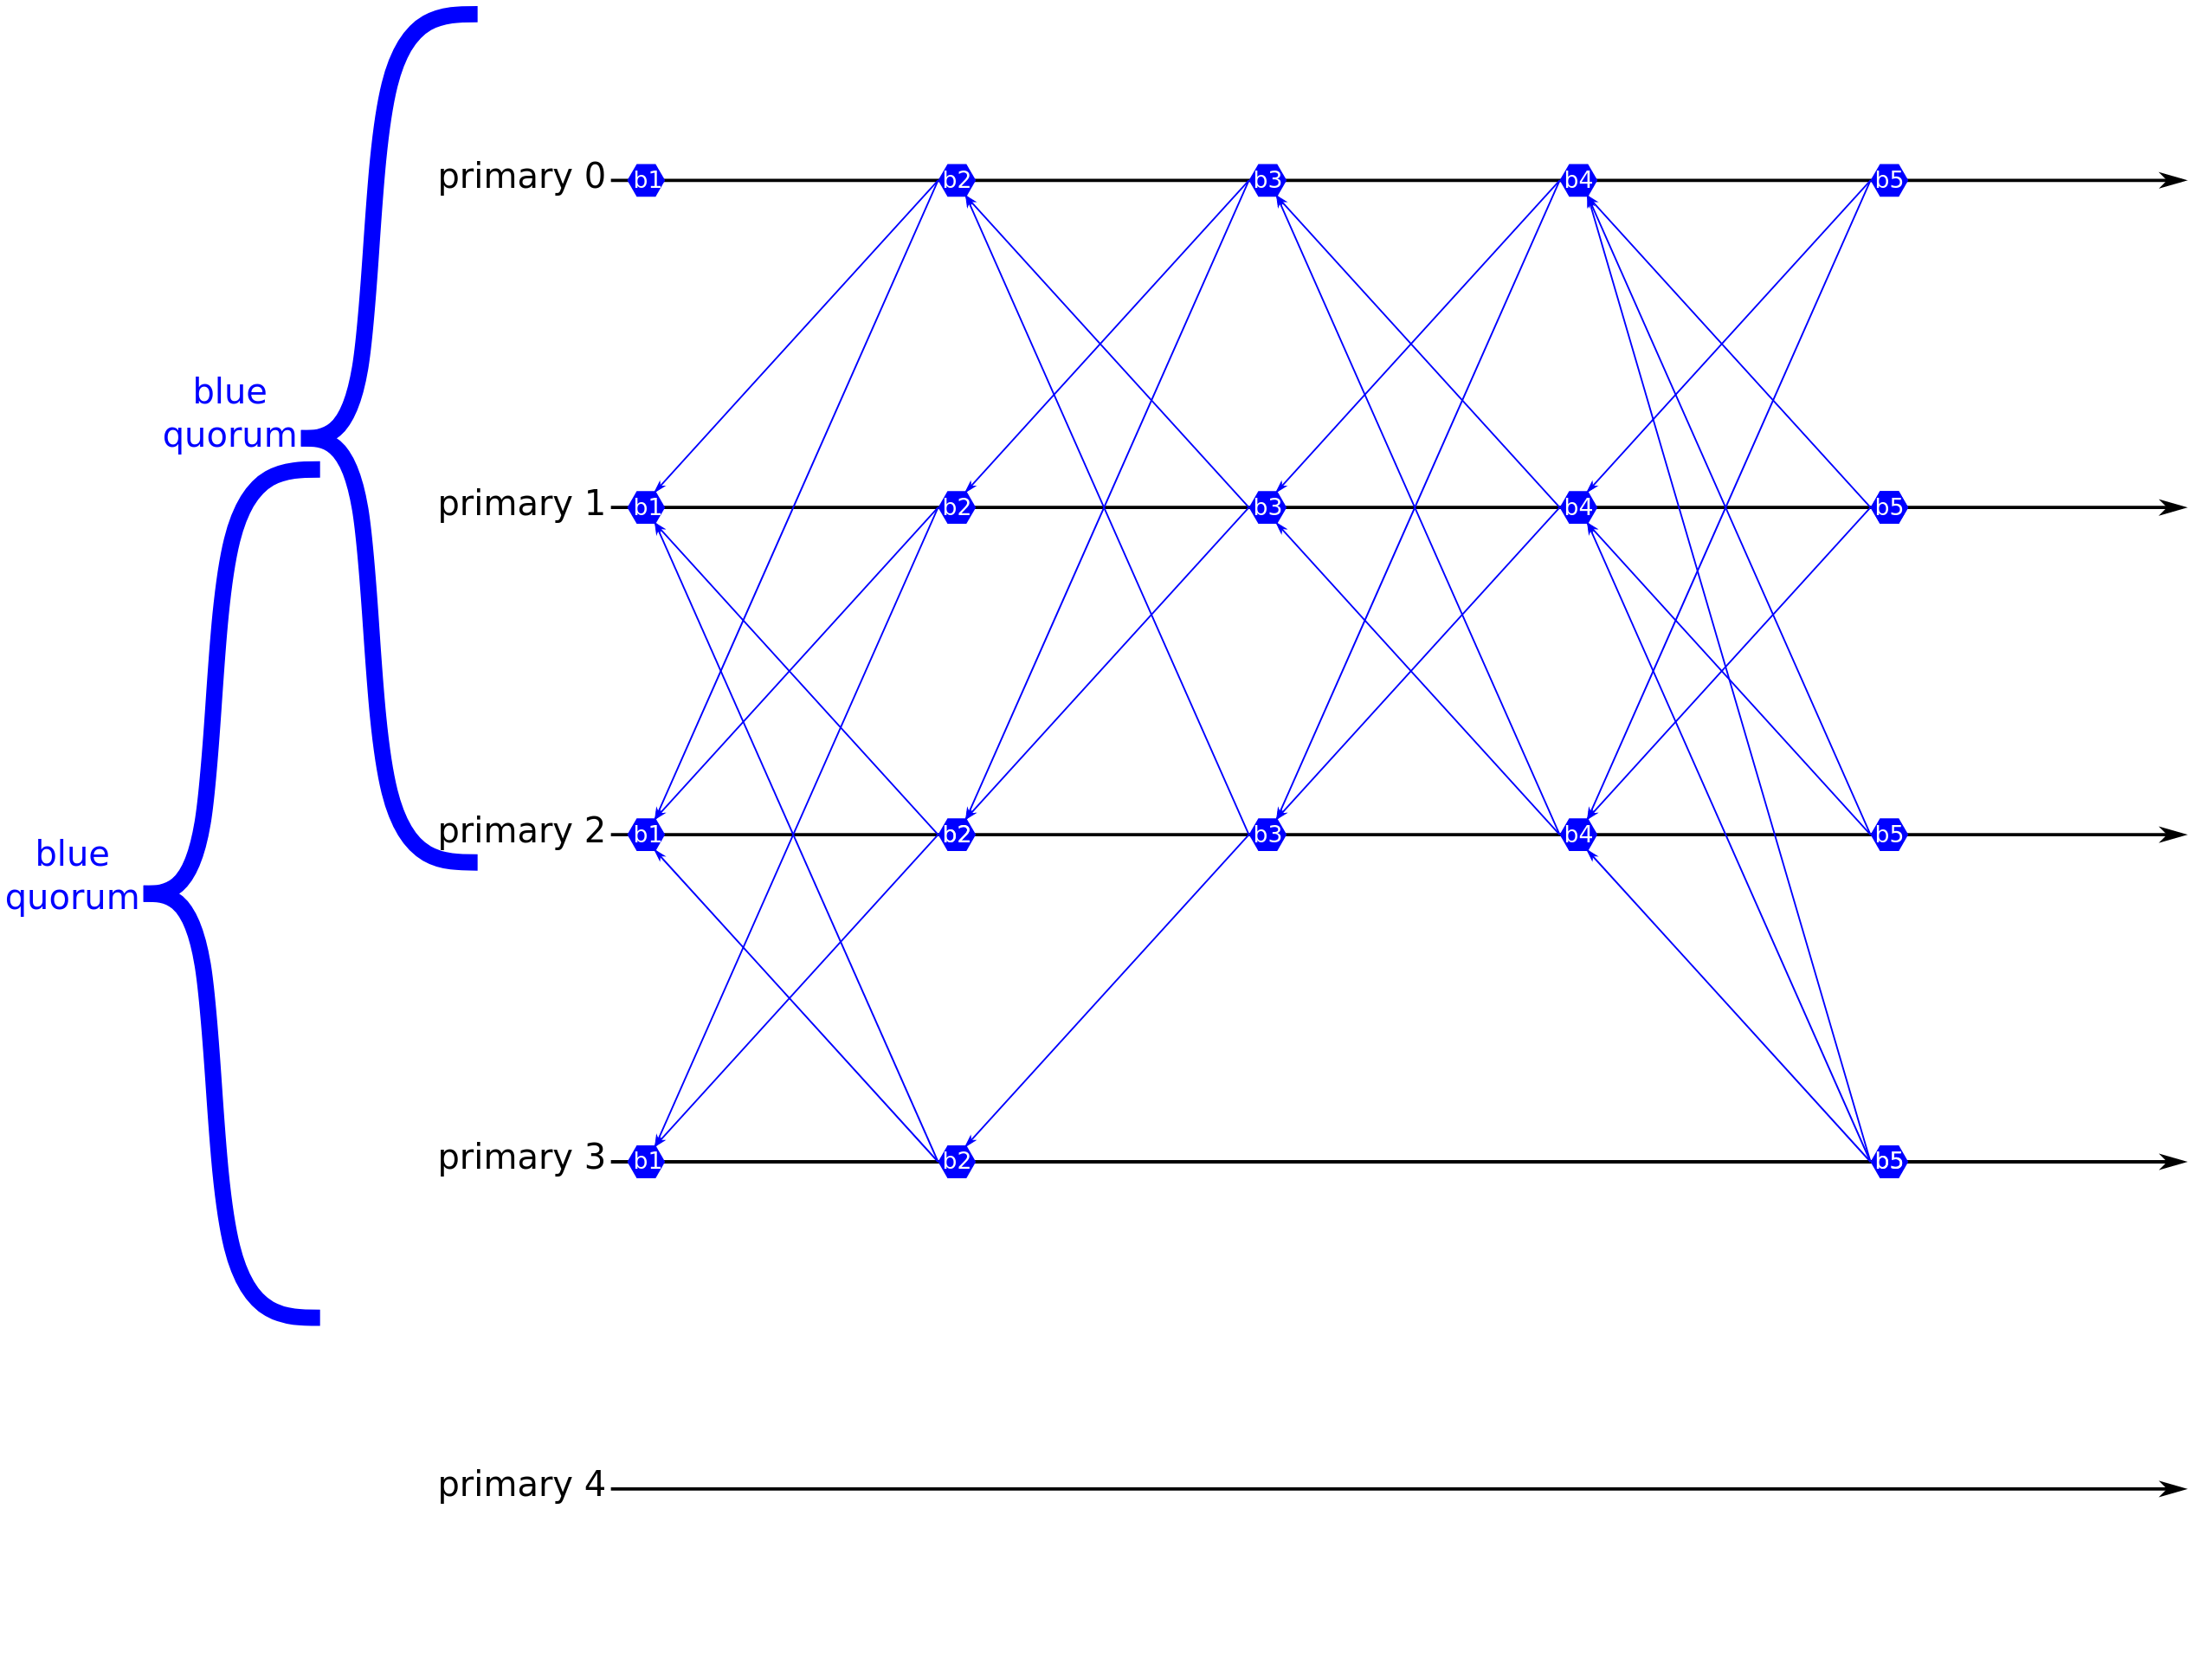
\includegraphics[width=.95\linewidth]{./blue_dag.png}
%   \caption{A mem-\Dag (self-references omitted)}
%   \label{fig:blue_dag}
% \end{figure}


% \begin{figure}[htb]
%   \centering
%   \begin{tikzpicture}
%     \node[draw] (avl) {transaction data};

%     \node[draw,right=1ex of avl] (dag) {“causal” \Dag structure};
%     \begin{pgfonlayer}{background}
%     \node (x) [fill=lightgray,fit=(avl)(dag)] {};
%   \end{pgfonlayer}
%   \node[above=2ex of x,draw,double] {uniqueness of headers};
% \end{tikzpicture}\makebox[0pt][r]{\Large \bf \color{blue} make this Fig. something that actually helps (or delete)} \protect\todo{where to put the signed quorums ?!}
%   \caption%
%   [Interdependence of availability and integrity]%
%   {Illustration of
%     the interdependence of the availability and
%     integrity protocols}
%   \label{fig:availability-n-integrity}
% \end{figure}



% Roughly, we have two complementary protocols running concurrently:
%  \begin{enumerate}
%  \item the availability protocol; and
%  \item the integrity protocol.
%  \end{enumerate}
%  The availability protocol makes sure
%  that transaction data is available
%  as long as necessary;\footnote{%
%    There is some fine print concerning
%    the conditions under which this is actually the case.
%  }
%  moreover,
%  the availability protocol
%  is tasked with keeping available
%  the \emph{signed headers},
%  \todo{explain \texttt{signed headers}}
%  which the integrity protocol produces.

%  The integrity protocol makes sure that
%  each validator can only produce one block in each of its (local) rounds.

% \end{comment}




\section{Architecture and communication patterns}
\label{sec:communication-patterns}
 \Hnr incorporates Narwhal's~\cite{NT}
 scale out architecture: %
 each validator has a unique \emph{primary} and %
 a number of \emph{workers} %
 (see \fig\ref{fig:validators}).



\begin{figure}[htb]
  \centering%\footnotesize
  \tikzsetnextfilename{scale-out-narwhal-architecture}
  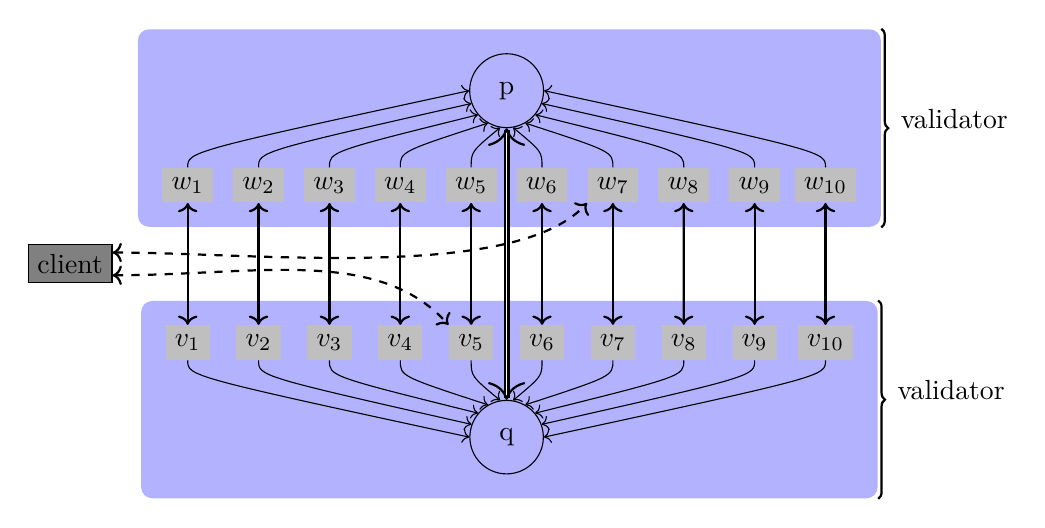
\begin{tikzpicture}[baseline={(p.south)},xscale=.9]
  \node[circle,draw,inner sep=1.5ex] (p) at (5.5,1.2) {p};
    \foreach \i in {1,...,10}{
      \coordinate (p_\i) at  (p.160+20*\i);
    }
    \foreach \i in {1,...,10}{
      \node[rectangle,fill=lightgray](w_\i) at (\i,0){\(w_{\i}\)};
      \draw[->] (w_\i.north) .. controls +(0,.2) .. (p_\i);
    }
    \begin{pgfonlayer}{background}
      \node[rounded corners,fill=blue!30!white,inner sep=2ex] (background) [fit=(w_1.south west)(w_10.south east)(p)] {};
      \draw[decorate,decoration={brace},thick] (background.north east)   -- node[anchor=base west] {~validator}(background.south east);
    \end{pgfonlayer}
    %%% 
    \begin{scope}[shift={(0,-2)},yscale=-1]
      \node[circle,draw,inner sep=1.5ex] (q) at (5.5,1.2) {q};
      \foreach \i in {1,...,10}{
        \coordinate (q_\i) at  (q.200-20*\i);
      }
      \foreach \i in {1,...,10}{
        \node[rectangle,fill=lightgray](v_\i) at (\i,0){\(v_{\i}\)};
        \draw[->] (v_\i.south) .. controls +(0,.2) .. (q_\i);
      }
      \begin{pgfonlayer}{background}
        \node[rounded corners,fill=blue!30!white,inner sep=2ex] (background) [fit=(v_1.north west)(v_10.north east)(q)] {};
        \draw[decorate,decoration={brace},thick] (background.north east)   -- node[anchor=base west] {~validator}(background.south east);
      \end{pgfonlayer}
    \end{scope}
    \path (w_1) -- (v_1) coordinate[pos=.5](zzz);
    \node[rectangle,fill=gray,draw,anchor=east] (c) at ([xshift=-7ex]zzz) {client};
    \begin{scope}[thick]
      \foreach \j in {1,...,10}
      \draw[<->] (v_\j) -- (w_\j);

      \draw[<->,dashed] (c.-15) .. controls +(2,0) and +(-1,1) .. (v_5.north west);
      \draw[<->,dashed] (c.15) .. controls +(2,0) and +(-1,-1).. (w_7.south west);
      \draw[<->,double] (p) -- (q);
    \end{scope}
   \end{tikzpicture}%
  \caption{The structure and communication patterns of validators}
  \label{fig:validators}
\end{figure}


\section{Worker actions (availability and executability)}
\label{sec:worker-actions}
Every validator has the same number of workers.
Thus,
each worker can be assigned a unique \emph{mirror worker}
on every other validator.
We shall adopt the convention
that  identifiers of mirror workers share the same subscript.
For example,
in \fig\ref{fig:validators},
workers~\(w_2\) and~\(v_2\) are mirror workers of each other.
Workers are mainly featuring in the availability protocol, %
which keeps the transaction available until execution. % 
Specifically,
workers keep track of (batches of) transactions,
their hashes,
and erasure coding shares---which shall be trivial, along the lines
of Narwhal and Tusk~\cite{NT}.
The core information that workers provide to their primaries  %
are hash references to transaction request data, %
besides consecutive batch numbers and some signatures. %
In this way,
primaries can save network bandwidth usage. %
Moreover,
as a secondary principle, %
primaries do not send messages %
or other direct signals to their workers.\xspace%
\footnote{%
  However, %
  workers receive signals upon successful execution of transactions, 
  which allows them to free up the transaction storage
  by executor nodes.
}%
\todo{add some short discussion about executor nodes, \etc \\
  also: is executor node still the right terminology ? 
}
\endnote{%
  Sharing the round number is the point where
  one might be tempted to deviate from the principle that
  validators never talk back to their workers
  (\emph{qua validator} -- the executor nodes on a validator do talk back).
}

\subsection{The pure availability protocol (pre-execution)}
\label{sec:base-protocol}
\endnote{%
  we now “announce” headers
  ---
  in contrast to what what is/was in the specs
  \tiny\tt(written March 7 2023, Tobias Heindel)
}


\todo{%
  at some point we discussed that
  \emph{worker hashes also should include an availability certificate %
  of the header creator's previous header} %
  \\
  However,
  as we now have the header announcement, %
  we have moved it to the primary's signature request
  \\
  double check ‼
}
\todo[inline,size=normalsize,color=green!80!black]{%
  defer all the data structure talk to the section on %
  message dependency management%
  Section/Appendix\ref{sec:mess-depend-manag}%
}
\todo[inline,size=normalsize,color=yellow!80!white]{
  \# issue:
  we are still missing information about 
  how long data has to be stored.
  We might want to have some executor node protocol here,
  deferring some details to 
  Section/Appendix\ref{sec:mess-depend-manag}
}
\begin{description}
\item[%
  \code{MessageEnum::TxReq}%
  Transaction request collection ({\tx}←)%
  ]
  \xnote{worker\\ ← client}
  \todo{in the typhon sources for \texttt{`heterogeneous\_narwhal`},
    each transaction collection is \emph{immediately} followed
    by a \texttt{TxAck}
  }
  Each worker keeps listening
  for incoming transaction requests from clients.\footnote{%
    The bandwith and amount of storage for storing incoming transactions 
    \emph{should} be big enough
    to process all incoming transactions.
    We share this assumption with Byzantine set consensus \cite{RedBelly}.
    Transaction fees are one way to avoid flooding attacks,
    making the latter prohibitively expensive.
    For example,
    we might consider using a \fifo-buffer; %
    however a priority queue that takes into account a combination of %
    fees and quality of service considerations %
    is more suitable for managing the flow of incoming transaction requests.
  }
  Transaction requests should be buffered using reasonably fast memory % 
  (to ensure that all requests are eventually served); %
  transaction request fees may be imposed %
  to control the rate of client requests. %
  \endnote{%
    The matter of reasonably fast transaction buffer
    needs additional context,
    possibly involving more specifics from the \ptop layer.
  }
  \begin{description}
  \item[%
    \code{???}%
    {Transaction batching (\(\txs:= \txs:\tx\))}%
    ]%
    \xnote{[worker]}%
    Every worker stores the received transaction request to %
    \emph{the} current batch \txs, %
    which is list of transaction requests. %
    % The worker adds the transaction request \tx to the current batch \txs. %
    This happens unconditionally,
    \ie there is always a unique current transaction batch 
    and every transaction request has to be added to the current batch. %
    New batches may be created over time, %
    but each batch in this “stream” of batches has a unique \emph{batch number}.
    Within a batch, %
    transactions are assigned consecutive {sequence numbers}: %
    the \emph{sequence number} of a transaction is 
    the position in the current batch. %
    Thus,
    each transaction request by identified by
    its \emph{batch}, \emph{sequence number} and the worker \textsc{id};
    we shall refer to this as the \emph{fingerprint} of the transaction
    request.\xspace%
    \footnote{%
      The order of transactions within a batch %
      might be permuted before execution %
      to avoid potential \mev. 
    }
  \item[%
    \code{TxToAll}%
    {Transaction broadcasting (\tx{}!\es{}⇒)}%
    ]%
    \xnote{%
      worker\\
      ⇒worker
    }%
    If a worker receives a transaction request, % 
    it will broadcast a copy to all mirror workers.
    In principle,
    we could use arbitrary erasure coding schemes.
    However,
    in line with the original version of Narwhal \cite{NT}, %
    we use full copies as erasure codes.
    Despite the coincidence of erasure codes and the “original” data, %
    we visually distinguish the “copy” of a transaction
    from the “original” transaction supplied by the client, 
    using two different symbols, namely \tx\ and \es, respectively. %
    When broadcasting copies of received transaction requests,
    the message also includes the fingerprint of the transaction request.
    \todo{and possibly time stamping information}
  \item[%
    \code{WHxToAll,WorkerHx}%
    {Worker hash broadcast (\tx{!}\wh{}↑⇒)}%
    ]%
    \xnote{worker%
      \\⇒ worker%
      \\→ primary%
    }
    When a worker receives a transaction request,
    this might trigger a new worker hash to be produced. %
    %(if it is “time”    to do so).
    In principle,
    the decision for when to send it is for the worker to decide %  
    (as long as each worker hash contains at least one transaction %
    and does not exceed a potential maximum size).\xspace%
    \footnote{%
      \label{fn:time}
      At which exact moment worker hashes are compiled can depend on several
      factors, 
      \eg on a maximum number of transaction requests per worker hash 
      or a maximum delay between the first and the last transaction request within a worker hash.
    } %

    {}\code{WorkerHashData,WorkerHashSignature}%
    The new worker hash consists of
    \begin{itemize}
    \item the hash of the current batch \txs, %
    \item the length of the current batch, %
    \item the identifier of the current worker, %
    \item a signature of the above data by the current worker. %
    \end{itemize}
    The worker hash broadcast involves the following steps: %
    \begin{enumerate}
    \item broadcasting the new worker hash to mirror workers; %
    \item sending the new worker hash to the worker's primary; %
    \item resetting the current transaction request buffer to the empty list; %
    \item incrementing the batch number; %
    \item last, but not least, %
      storing the transactions of the current batch for retrieval. %
      \todo{%
        The present state of the specs (in flux),
        we notify workers for matters of executing at the level of single transactions
      }
    \end{enumerate}%

  \item[\code{MessageEnum::TxAck}
    Transaction request acknowledgment]
    Optionally, %
    one may acknowledge the client's requests. 
    \todo[inline,size=normalsize,color=SkyBlue]{%
      In the
      \href{https://github.com/anoma/typhon/tree/hnarwhal-stateright/hn-stateright/heterogeneous_narwhal}%
      {code},
      we instantly acknowledge each received transaction
      by sending a message back to the sender of the transaction request.
    }
  \end{description}
  \endnote{%
    If we want to perform proper erasure coding,
    we also have to replace a full broadcast by
    something more sophisticated.
    \Eg each mirror worker receives a different message.
    We first cover the case of trivial erasure coding
    ‼[covering the case of proper erasure codining in ‽].
  }

\item[%
  \code{MessageEnum::TxToAll}%
  Transaction copy (\es{}←)%
  ]\xnote{%
    worker\\
    ←worker
  }%
  \todo{move to appendix / message dependency managment:\\
    For the proper handling of transaction copies and worker hashes
  of mirror workers,
  we keep for each mirror worker
  a set of \emph{active batch numbers}
  and a map from active batch numbers to
  a set of (ranges of) sequence numbers of received transactions in that batch,
  paired with a worker hash option,
  depending on whether or not we have received the corresponding worker hash.
  }
  Upon receiving a transaction copy, %
  the worker has to store the copy locally %
  such that its hash can be retrieved quickly via its fingerprint, \ie
  \begin{itemize}
    \item the \textsc{id} of the collecting worker, 
    \item the batch number of the batch to which it belongs, and
    \item the sequence number within the batch to which it belongs.
    \end{itemize}
    Note that copies of transactions are \emph{not} signed by the worker. %
    Signatures are deferred to worker hash broadcast. % 
    Storing transaction copies as above will be useful %
    for handling “foreign” worker hashes, %
    \ie worker hashes that refer to transactions that are collected at other
    workers. 
    \begin{description}

  \item[\code{WHxFwd}{Worker hash forwarding (\es!\wh[]↑)}] 
    \xnote{%
      worker\\
      →primary%
    }
    In case, %
    the transaction was the last missing one to match a previously received worker hash, %
    the worker hash is send to its primary.
    The (pre-)condition\xspace%
    \todo{%
      This terminology clashes. What else? 
      “triggering condition” ?!
    } is that all transactions that are referenced in the worker
    hash have already been received and stored.\xspace%
    \footnote{%
      This might be unexpected order of events,
      but the sending of transaction data might be “delayed”. 
    } 
  \end{description}

% \item[Worker hash compilation (\wh)]
%   \xnote{(worker)}
%   Towards the end of a “validator round”,\endnote{%
%     Is there any such thing as “validator round”?\\
%     - sequence number\\
%     - validator height\\
%     - ...
%   }%
%   \todo[inline,size=normalsize,color=red,caption={}]{%
%     here now, we need to
%     \begin{enumerate}
%     \item introduce signals from primary to workers,
%     \item replace the round number by a “take” based mechanism
%     \end{enumerate}
%   }
%   \xspace
%   each worker produces its worker hash for the broadcast batch of transactions.
%   In detail,
%   a worker hash consists of
%   \begin{itemize}
%   \item the hash of the broadcast list of transactions,
%   \item the number of transactions, and
%   \item the \st{round number}\ul{take},
%     \todo[color=SkyBlue]{%
%       very much like in a movie,
%       we piece together each header form \textsc{take},
%       or any other single word for \emph{batch number}
%       }
%   \end{itemize}
%   signed by the worker.
%   \endnote{\color{red}
%     For general erasure coding:
%     \em Does this need to includes for each receiving worker,
%     the (hashes of the) erasure coding shares that
%     they should have available. ?
%   }

\item[%
  \code{WHxToAll}%
  Worker hash reception ({\wh[]←})%
  ]%
  \xnote{%
    worker\\%
    ← worker%
  }
  When a worker receives a worker hash from a mirror worker %
  there are two cases:
  either it has already has received all the referenced transaction copies
  (and can forward the worker hash to its primary) 
  or it has to store the worker hash
  (and the worker hash forwarding will be triggered by the last transaction
  copy).\endnote{%
    Well, and how long are we gonna wait for missing transactions of worker hashes?
  }
  \begin{description}
  \item[%
    \code{MessageEnum::WHxFwd}%
    Worker hash forwarding ({\wh[]!\wh[]↑})%
    ]
    \xnote{worker\\ → primary} 
    If a worker has already stored the transactions of a received worker hash, %
    it sends the worker hash to its primary.\footnote{%
      Validators will use this information
      to send availability commitments to block headers of other primaries.
    }
  \end{description}
\end{description}

We have described the protocol in terms of %
what workers do in reaction to \emph{receiving} messages. %
This emphasizes that sending a message might be due to several, slightly
different types of scenarios %
(depending of which message from a \emph{set} of triggering messages arrives
last and thus becomes {the} final trigger). %


\begin{figure}[htb]
  \centering
  \todo[inline,size=normalsize,caption={}]{%
    \begin{itemize}
    \item need to “fix” the \tx subscripts to be sequence numbers;
      possibly adding also the batch number of the worker hash?
    \item header announcements only need to send “fingerprints” of headers,
      for the moment represented by \(\wh[]^*\)
    \end{itemize}
  }
  %
  \tikzstyle{every node}+=[outer sep=0pt,inner sep=1pt]
  \newcommand{\primaryDistance}{15ex}
  \newcommand{\workerPrimaryDistance}{1ex}
  \newcommand{\workerDistance}{3ex}
  \scalebox{.9}{%
  \footnotesize%
  \tikzsetnextfilename{availability-protocol-at-genesis}
  \begin{tikzpicture}[scale=1.2]
    %%%%%%%%%%%%%%%%%%%%%%%%%%%%%%%%%%%%%%%%%%%%%%%%%%%%%%%%%%%%%%%%%%%%%%%%%%%%%%%%
    % The message passing diagram of the availability protocol at genesis
    %%%%%%%%%%%%%%%%%%%%%%%%%%%%%%%%%%%%%%%%%%%%%%%%%%%%%%%%%%%%%%%%%%%%%%%%%%%%%%%%
    % first the time lines for primaries and their workers
    \coordinate (primaryAnchor) at (0,0);
    \foreach \p in {1,...,5} {
      \node[below=\primaryDistance of primaryAnchor,anchor=east] (p\p)
      at (primaryAnchor) {\ensuremath{\text{primary}_\p}};
      \draw[->] (p\p) -- ++(10.4,0);
      \coordinate (workerAnchor) at ([yshift=-\workerPrimaryDistance]p\p.east);
      \foreach \j in {1,...,2} {
        \node[below=\workerDistance of primaryAnchor,anchor=east] (w\p_\j)
        at (workerAnchor) {\ensuremath{\text{worker}_{\p,\j}}};
        \draw[->,draw=lightgray,semithick] (w\p_\j) -- ++(10.4,0) ;
        \coordinate (workerAnchor) at (w\p_\j.east);
      }
      \coordinate (primaryAnchor) at (p\p.east);
    }
    %%%%%%%%%%%%%%%%%%%%%%%%%%%%%%%%%%%%%%%%%%%%%%%%%%%%%%%%%%%%%%%%%%%%%%%%%%%%%%%%
    % a first transaction tx1
    \node (tx1) at ([xshift=3.5ex]w1_1.east) {\tx₁};
    \draw[->,double,dotted,shorten >=-2ex] (tx1.200) ++ (200:1em) -- (tx1);
    \foreach \p in {2,...,5} {
      \node (es\p_1) at ([xshift=6ex-\p ex]tx1|-w\p_1) {\es₁};
      \draw[->] (tx1) -- (es\p_1) ;
    }
    % a bunch of transactions tx2-5 that will make it into WHs actually
    \node (tx2) at ([xshift=3*3.5ex]w3_2.east) {\tx₂};
    \draw[->,double,dotted,shorten >=-2ex] (tx2.200) ++ (200:1em) -- (tx2);
    \foreach \p in {1,2,4,5} {
      \node (es\p_2) at ([xshift=6ex-\p ex]tx2|-w\p_2) {\es₂};
      \draw[->] (tx2) -- (es\p_2) ;
    }
    \node (tx3) at ([xshift=5*3.5ex]w3_2.east) {\tx₃};
    \draw[->,double,dotted,shorten >=-2ex] (tx3.200) ++ (200:1em) -- (tx3);
    \foreach \p in {1,2,4,5} {
      \node (es\p_3) at ([xshift=6ex-\p ex]tx3|-w\p_2) {\es₃};
      \draw[->] (tx3) -- (es\p_3) ;
    }
    \node (tx4) at ([xshift=7*3.5ex]w3_1.east) {\tx₄};
    \draw[->,double,dotted,shorten >=-2ex] (tx4.200) ++ (200:1em) -- (tx4);
    \foreach \p in {1,2,4,5} {
      \node (es\p_4) at ([xshift=6ex-\p ex]tx4|-w\p_1) {\es₄};
      \draw[->] (tx4) -- (es\p_4) ;
    }
    \node (tx5) at ([xshift=9*3.5ex]w3_1.east) {\tx₅};
    \draw[->,double,dotted,shorten >=-2ex] (tx5.200) ++ (200:1em) -- (tx5);
    \foreach \p in {1,2,4,5} {
      \node (es\p_5) at ([xshift=6ex-\p ex]tx5|-w\p_1) {\es₅};
      \draw[->] (tx5) -- (es\p_5) ;
    }
    % collection of txs into worker hashes wh1 and wh2
    \node[right=.1ex of tx5] (wh1) {\wh₁};
    \draw[dotted,bend right=2.5ex] (wh1.center) to (tx5.center);
    \draw[dotted,bend right=5ex] (wh1.center) to (tx4.center);
    \node[right=3.5ex of wh1|-tx3] (wh2) {\wh₂};
    \draw[dotted,bend left=2.5ex] (wh2.center) to (tx3.center);
    \draw[dotted,bend left=5ex] (wh2.center) to (tx2.center);
    %%%%%%%%%%%%%%%%%%%%%%%%%%%%%%%%%%%%%%%%%%%%%%%%%%%%%%%%%%%%%%%%%%%%%%%%%%%%%%%%
    % "upload" of worker hashes wh1 and wh2 to the primary, wh1' and wh2'
    \node (wh1') at ([xshift=-2ex]wh2|-p3) {\wh₁};
    \draw[->] (wh1) -- (wh1');
    \node[right=0ex of wh1'] (wh2') {\wh₂};
    \draw[->] (wh2) -- (wh2');
    % the following should be much later, but ... (unique harmless hack)
    \node[right=1ex of wh2',fill=white] (hd3) {{\hd[]}};
    \foreach \k in {1,2}
    \draw[dotted,bend right=9ex-3*\k ex] (hd3) to (wh\k'.center);
    %%%%%%%%%%%%%%%%%%%%%%%%%%%%%%%%%%%%%%%%%%%%%%%%%%%%%%%%%%%%%%%%%%%%%%%%%%%%%%%%
    % dissemination of worker hashes wh1 and wh2
    \foreach \p in {1,2,4,5} {
      \node (wh1_\p_1) at ([xshift=3ex-\p ex]wh1'|-w\p_1) {\wh[]₁};
      \draw[->] (wh1) -- (wh1_\p_1) ;
    }
    \foreach \p in {1,2,4,5} {
      \node (wh2_\p_2) at ([xshift=6ex-\p ex]wh2'|-w\p_2) {\wh[]₂};
      \draw[->] (wh2) -- (wh2_\p_2) ;
    }
    %%%%%%%%%%%%%%%%%%%%%%%%%%%%%%%%%%%%%%%%%%%%%%%%%%%%%%%%%%%%%%%%%%%%%%%%%%%%%%%%
    % worker hash upload at receiving validators
    \foreach \whx in {1,2} { % for each of the two worker hashes
      \foreach \p in {1,2,4,5} { % for each "other" validator
        \node (wh\whx_\p_\whx') at ([xshift=4ex-\whx ex]wh\whx_\p_\whx|-p\p) {\wh[]\ensuremath{{}_\whx}};
        \draw[->] (wh\whx_\p_\whx) -- (wh\whx_\p_\whx');
        % and header creation (after second block)
        % ... and sending availability votes
        \ifthenelse{\equal{\whx}{2}}%
        {\node[right=2ex of wh\whx_\p_\whx',fill=white,draw=none] (hd\p) {\({\hd[]}^*\)};
          \foreach \k in {1,2}
          \draw[dotted,bend right=9ex-3*\k ex] (hd\p) to (wh\k_\p_\k'.center);
        }%
        {}%
      }
    }
    %%%%%%%%%%%%%%%%%%%%%%%%%%%%%%%%%%%%%%%%%%%%%%%%%%%%%%%%%%%%%%%%%%%%%%%%%%%%%%%%
    % collect "foreign" whs into availability votes for a block
    \coordinate (ac) at ([xshift=2ex,yshift=2ex]hd1|-p3);
    \foreach \p in {1,2,4} { % for each "other" validator
      \node[fill=white] (av\p) at (ac){{\hd[]}\makebox[0pt][l]{\ensuremath{{}_{\sim\p}}}};
      \coordinate (ac) at ([xshift=-1ex,yshift=-1ex]ac);
    }
    \foreach \p in {1,2,4} { % for each "other" validator
      \draw[->] (hd\p) -- (av\p.east);
      \draw[%ultra thick,red,double,
      ->] (hd3) --
      % node[auto]{trigger}
      (hd\p);
    }
    \draw[%ultra thick,red,double,
    ->] (hd3) --%node[auto]{trigger} 
    (hd5);
    \node[fill=white] (av3) at (ac){{\hd[]}\makebox[0pt][l]{\ensuremath{{}_{\sim3}}}};
    \draw[->] (hd3) -- (av3);
    \begin{pgfonlayer}{background}
      \node[fit={(av3)(av1)([xshift=2ex]av1.north east)},fill=lightgray] (ac3) {};
    \end{pgfonlayer}
    % broadcast the availability certificate
    \foreach \p in {1,...,5} { % for each "other" validator
      \node (ac\p') at ([xshift=17ex-\p ex]ac|-p\p) {\ac\ensuremath{{}_\p}};
      \draw[->] ([yshift=2.5ex-\p ex]ac3.east) -- (ac\p');
    }
  \end{tikzpicture}%
  }
  \caption{The availability protocol in the genesis round}
  \label{fig:availability-protocol}
\end{figure}


\todo[inline,size=normalsize]{%
  so, signed qourums are an “output” of the integrity protocol,
  and need to be made available
  (such that it is possible to create new headers).
  NEEDS EXPLAIN
}

\todo[caption={}]{%
  concerning “triggering” the header construction,
  there are the following points
  \\
  1. when a the triggering signing request is \emph{received} by a primary,
  we might need to “wait” for the corresponding worker hashes
  \\
  2. new signing for more recent rounds make old ones obsolete
  \\
  3. what are the incentives for speedy signing ?
}\endnote{%
  On speedy signing incentives:
  \begin{itemize}
  \item as a validator, I want primarily \emph{my} blocks signed
  \item
    So, why should I sign \emph{your} header?!
    \begin{itemize}
    \item It comes even with the storage commitment for my workers!
    \item Actually, if “everybody” else is signing, I am still gonna be fine !!!
    \end{itemize}

    Thus, having a signature as part of an availability certificate should give
    some kind of reward!
  \end{itemize}
  On the other hand,
  it is natural to collect signatures for the availability certificate
  on a “first come, first served” basis
}




\subsection{Execution support protocol}
\label{sec:exe-supp-protocol}

\todo{todo!}
\section{Primary actions}
\label{sec:primary-actions}

Primaries will follow a protocol %
in which we can distinguish between matters of availability %
and matters of integrity. %
For the availability protocol,
we shall treat first the special case at genesis 
and later describe the additional (re-)actions
in the typical mode of operation. %
The integrity protocol is described in between the two; %
after all, the two protocols are closely intertwined.\xspace%
\footnote{%
  Specifically, %
  the integrity protocol produces blocks, %
  and signed quorums of these are necessary for block headers (after genesis); %
  however, %
  header announcement and signing are part of the availability protocol. %
}

In the protocol description for validators, %
we avoid copying text if a message has several triggers
by simply listing the alternative triggers of a message
(after the “default” trigger).
For the pure availability protocol for workers,
this would lead to a single heading
for worker hash forwarding.
\begin{center}
  \bf{Worker hash forwarding (\((\wh[] / \es)\)!\wh↑)}
\end{center}
So,
the primary trigger for worker hash forwarding are worker hashes,
but transaction copies are alternative triggers  %
(in cases of message delay irregularities). %


\subsection{Availability at genesis}
\label{sec:avail-at-genes}




\begin{description}
\item[\code{WorkerHx}Worker hash completion (\wh←)]
  \xnote{%
    primary\\
    ←worker
  }%
  When a worker hash (that was compiled by a local worker) is received,
  the primary adds the worker hash to the current list of worker hashes \whs.

  \begin{description}
  \item[\code{NextHeader}{Header announcement (\wh!\hd[]⇒)}]%
    \xnote{%
      primary \\
      ⇒primary
    }
    The primary may announce the next header %
    (if the primary considers it is “time” to do so---cf.\ Footnote~\ref{fn:time}).
    The genesis header consists of
    the current list of worker hashes,
    tagged with the identifier of the primary;
    the round number zero is implicit.
    The message of the batch announcement only contains
    the \emph{fingerprint} of a header, namely 
    \begin{itemize}
    \item the identifier of the primary
    \item a list of pairs of a batch number and a worker \textsc{id}.
    \end{itemize}
    The actual header itself consists of
    \begin{itemize}
    \item the identifier of the primary and
    \item the list of worker hashes. 
    \end{itemize}

  \end{description}

% \item[Genesis header compilation ({\hd[]})]
%   \xnote{[primary]}
%   If a primary has obtained a “complete set”
%   \todo{
%     \emph{“complete set”}
%     is an undefined term, right?
%     }%
%     of
%   worker hashes for the genesis round
%   from its workers,
%   it can compile a block header.
%   Compiling worker hashes into headers
%   works the same for worker hashes of local workers
%   and those generated from transactions received at other validators.%
%   \footnote{%
%     However,
%     the compiled worker hashes will have different roles,
%     depending on whether they are stemming from local workers or not.
%     In particular,
%     primaries will only need to generate
%     certificates of availability for “local” headers.
%   }
%   At genesis,
%   each header consists of
%   \begin{itemize}
%   \item the creator's identity and
%   \item and the list of worker hashes.
%   \end{itemize}
%   \begin{description}
%   \item[Header announcement / Signature request]
%     A primary announces the next \emph{header}
%     by sending information about
%     \begin{itemize}
%     \item information about which worker hashes to be included
%       (as pairs of worker-ids and batch numbers)
%     \item the round number
%     \end{itemize}
%     \todo[inline,size=normalsize]{it is, isn't it?}
%     .
%   \item[Header collection]
%     The primary has to collect
%   \end{description}


\item[{\code{WorkerHx}Worker hash reception (\wh[]←)}]
  \xnote{%
    primary\\
    ←worker
  }%
  When a worker hash that stems from a worker on a different validator is received, %
  the primary adds the worker hash to the current list of known worker hashes. %
  % Primaries keep a set of \emph{active} worker hashes for each validator %
  % and also a set of worker hash fingerprints. %

  \begin{description}
  \item[{Header signature commitment (\wh[]!\(\hd_{\sim}\)→)}] %
    \xnote{primary\\
      →primary
    }
    If the received worker hash completes the list of known worker hashes
    to match a previously received header fingerprint, %
    the primary commits to the header by 
    signing the header
    and sending the signed header back to the creator of the header. %
    % We can now free the memory for the fingerprints \etc
    % (or wait until the certificate of availability has been received in response
    % to the commitment).
    % \todo{which one is the proper choice ?}
  \end{description}


% \item[Availability voting/commitment (\hdₚ→)]
%   \xnote{primary\\ → primary}
%   A genesis header of a primary is acceptable
%   if all its worker hashes have been forwarded
%   by the local workers
%   (which are trusted to have checked these worker hashes).
%   The latter implies that the relevant erasure coding shares
%   are kept available.
%   An availability commitment is made
%   by signing the header
%   and sending the signed header to the creator
%   (for the purpose of aggregation into availability certificates).

\item[{Header announcement (\(\hd[]^*\)←)}] %
  \xnote{%
    primary\\
    ←primary
  }
  If the primary receives a header fingerprint from a another primary, %
  it is stored as long as the header might still be included into some learner-specific \Dag. %
  \todo{double check the “livetime”}
  We also elide to mention that each correct validator has to check whether the
  received data are consistent with the local observations. 

  \begin{description}
  \item[{Header signature commitment (\(\hd[]^*!\hd_{\sim}\)→)}] %
    \xnote{%
      primary\\
      →primary
    }
    If all worker hashes of the received header fingerprint are known to the primary, 
    the primary commits to the header by answering with a signature over the
    header. 
  \end{description}

  \todo[inline,size=normalsize]{%
    ideally, a  “flowchart” would get rid of the “code duplication” !!!%
    \\
    also, a dependency graph with “joint” triggering 
    would be rather useful (to convey the main ideas)
  }

\item[Header signature (\hdₚ←)]
  \xnote{%
    primary\\
    ←primary
  }
  The signature of a received availability commitment
  is either stored or added to the aggregated signature “under construction”,
  leading towards a certificate of availability. %
  If the received signature completes a global quorum, %
  it triggers the broadcasting of %
  the completed aggregated signature, %
  \ie the certificate of availability. % 

  \begin{description}
  \item[{Availability certificate broadcast %
      (\hdₚ!\ac⇒)}
    ]
    \xnote{primary\\
      ⇒primary
    }
    If the received commitment completes a global weak quorum for
    its genesis header,
    it broadcasts the certificate of availability. 
  \end{description}

% \item[optional header distribution]
%   ~\todo[inline,size=normalsize]{%
%     Right now,
%     there seems no reason to add this “safe guard”;
%     it might be confusing.
%   }
%   One might expect that header creators send their headers around.
%   However,
%   there is no need for this.%
%   \endnote{... at least in theory, we'll keep it slick for the moment}
 
  % has uploaded a worker hash
  % for the genesis round,
  % optionally,
  % the primary \emph{can} distribute
  % the genesis header:
  % ‼{\color{red} why do we do this then at all?}
  % \begin{itemize}
  % \item the primary~\(p\)
  % \item worker hashes \(\wh_1 \cdots \wh_n\),
  %   produces by the local workers at \(p\)'s validator.
  % \end{itemize}
  % In theory,
  % this step is not necessary,
  % since each other primary will eventually receive
  % the  worker hashes \(\wh_1 \cdots \wh_n\), 
  % forwarded from it's workers.
 
  % Note,
  % the creating primary of the header does not sign it;
  % the signature is “delayed” until
  % enough primaries have commited to storing
  % the underlying data,
  % as described by the next action.

  % ‼[a “sequence number” with the set of “target” learners should suffice,
  % to trigger such an header request]
\end{description}

A (partial) execution of the availability protocol at genesis is
illustrated in \fig\ref{fig:availability-protocol}.
Also, %
note that in some exceptional circumstances,
a received header signature \(\hdₚ\) might also need 
action according to the integrity protocol,
as explained next. 


\todo[inline,size=normalsize,caption={}]{add flow charts for
  \begin{enumerate}
  \item workers
  \item primaries
  \end{enumerate}
}

\FloatBarrier


\subsection{Integrity: the general case at once}
\label{sec:integr-gener-case}
First off,\todo{mention the two ways of interleaving:\\
  - re-use of signatures\\
  - additional new data to be kept available
}
the integrity-protocol re-uses the sending of signed headers~\(\hdₚ\) to the creator
(from the availability-protocol)
as a commitment of the signer to
one unique header for the  validator (and round),
namely the first one signed and sent.
Thus,
correct validators will not sign and send any other header
from the creator of the header (for the same round).

\paragraph{Integrity signing}
  \xnote{⚠}
  \emph{Signing and sending a header to its creator implies that
  (a correct) primary will not sign any other header
  of the same creator with the same round number. %
  (Recall that the headers at genesis implicitly are of round zero.) %
}

\todo[inline,size=normalsize]{a mess for the poor reader that has never heard of integrity
  vs. availability ⁈}

The availability protocol for primaries will use
counterparts to blocks in Narwhal~\cite{NT}, %
which come with  references to a quorum of blocks,   
namely \emph{learner-specific blocks} 
and \emph{signed block quorums}, defined as follows:  
a \emph{learner-specific block} is a block header signed by a learner-specific quorum
and a \emph{signed quorum} is a quorum of blocks signed by a primary.
Finally,
a \emph{typical header},
\ie one after genesis,
consists of
\begin{itemize}
\item the identifier of a primary 
\item a list of worker hashes
\item an availability certificate for the previous header of the same primary
\item the round number 
\item a non-empty\todo{discuss with isaac} list of signed quorums,
  at most one per learner. 
\end{itemize}
The first two items were already present in genesis block headers
while the remaining three only come into play in later rounds. 
With these definitions in place,
we can describe the primary actions in the availability protocol. 


\begin{description}
\item[Header signature (\hdₚ←)]
  \xnote{%
    primary\\
    ←primary
  }
  If the received signature of a header
  (interpreted as {integrity commitment})
  completes a full 
learner-specific quorum of signatures, 
  the received signature triggers the broadcast of one (or several) learner-specific blocks.

\todo{fix inline blocks (see \LaTeX source)}
% \begin{verbatim}
% \usetikzlibrary {shapes.symbols}
% \begin{tikzpicture}
%   [every node/.style={signal, draw,  text=white, signal to=nowhere}]
%   \node[fill=green!65!black, signal to=east] at (0,1) {To East};
%   \node[fill=red!65!black, signal from=east] at (0,0) {From East};
% \end{tikzpicture}
% \end{verbatim}
  \begin{description}
  \item[Block broadcast (\hdₚ!\((\bk⇒)^+\))]
    \xnote{%
      primary \\
      ⇒ primary
    }
    If the received header signature 
    %The aggregated signatures of a block header lead to completion of
    completes a \emph{learner-specific} block, 
    for each such new block, %
    the signature aggregator will broadcast a block
    to all primaries that belong to some quorum of the respective
    learner.\footnote{%
      In other words, 
      the broadcast is to  all primaries in the union of all quorums of
      the respective learner. 
    }
    The (learner-specific) round number of a (learner-specific) block 
    is derived from the block header that it is based on: 
    \todo{double check the following with isaac}%
    it defaults to zero, 
    unless there is a signed quorum that is the last one for the respective learner
    in the chain of block headers of the same primary
    and
    then it is one plus the signed quorum's round number.\xspace%
    \footnote{%
      Signed quorums will be used as references to previous blocks in %
      the learner-specific \Dag[s],
      as detailed in Section/Appendix\ref{???}. %FIXME reference.
    }
    \todo{fill in reference}
  \end{description}

\end{description}
Note that there is no conceptual difference between
the integrity protocol at genesis,
compared to the typical case.
The only difference is that headers need to carry 
additional information.
Now, 
we can finish the description of heterogeneous Narwhal,
by filling in the missing detail of the availability-protocol after genesis
(see also \fig\ref{fig:data-structures},
for the difference between headers at genesis and afterwards).
\todo{we need to explain some place the difference in (possibly) using weak links }


\begin{figure}[htb]
  \centering
  \tikzstyle{every node}+=[outer sep=0pt,inner sep=1pt]
  \newcommand{\primaryDistance}{15ex}
  \newcommand{\workerPrimaryDistance}{1ex}
  \newcommand{\workerDistance}{3ex}
  \scalebox{.8}{%
    \footnotesize%
    \tikzsetnextfilename{integrity-protocol}
    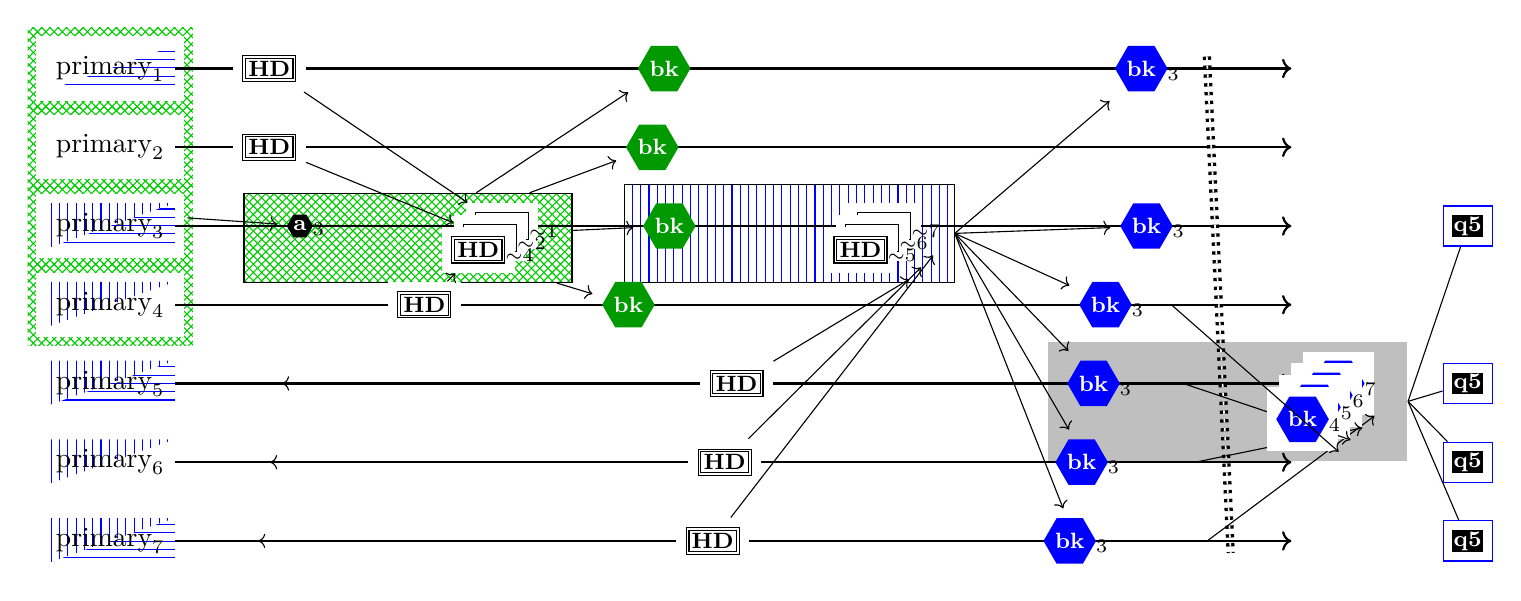
\begin{tikzpicture}[scale=1,thick]
      %%%%%%%%%%%%%%%%%%%%%%%%%%%%%%%%%%%%%%%%%%%%%%%%%%%%%%%%%%%%%%%%%%%%%%%%%%%%%%%%
      % The message passing diagram of the integrity protocol
      %%%%%%%%%%%%%%%%%%%%%%%%%%%%%%%%%%%%%%%%%%%%%%%%%%%%%%%%%%%%%%%%%%%%%%%%%%%
      \coordinate (primaryAnchor) at (0,0);
      \foreach \p in {1,...,7} {
        \node[below=\primaryDistance of primaryAnchor,anchor=east] (p\p)
        at (primaryAnchor) {\ensuremath{\text{primary}_\p}};
        \draw[->] (p\p) -- ++(15,0);
        \coordinate (primaryAnchor) at (p\p.east);
      }
      \begin{pgfonlayer}{background}
        \foreach \p in {1,...,4}{
          \node[pattern=crosshatch, pattern color=green!80!black,fit={(p\p)},inner sep=1.5ex] {};
          \node[fill=white, fit={(p\p)}] {};
        }
        \foreach \p in {1,3,5,7}{
          \fill[pattern=horizontal lines, pattern color=blue]
          (p\p.north east) -- (p\p.south west) -- (p\p.south east) -- cycle;
        }
        \foreach \p in {3,...,7}{
          \fill[pattern=vertical lines, pattern color=blue]
          (p\p.north east) -- (p\p.south west) -- (p\p.north west) -- cycle;
        }
      \end{pgfonlayer}

      \node[inner sep = 4ex] (theOrigin) at ([xshift=-3ex]p3.10) {};
      \foreach \p in {1,...,7} { % for each "other" validator
        \coordinate (ac\p') at ([xshift=17ex-\p ex]theOrigin|-p\p) ;
    }
    \node (ac3') at ([xshift=17ex-3 ex]theOrigin|-p3) {\ac\ensuremath{{}_3}};
    \draw[->] (theOrigin) -- ([xshift=4ex,yshift=4ex]ac3');
    \coordinate[right=14ex of ac3'] (sigAgg);
    \foreach \p in {1,2,4} { % for each "other" validator
      \node[fill=white] (av\p) at (sigAgg){\hd\makebox[0pt][l]{\ensuremath{{}_{\sim\p}}}};
      \coordinate (sigAgg) at ([xshift=-1ex,yshift=-1ex]sigAgg);
    }
    \foreach \p/\y in {1/2,2/1,4/-14} {
      \node[left=\y ex of ac\p',fill=white] (hd\p') {\hd};
      \draw[->] (hd\p') -- (av\p);
    }
    \begin{pgfonlayer}{background}
     
      \node[fit={(av4)([xshift=2ex]av1.north east)([xshift=-2ex]ac3'.west)},pattern=crosshatch,pattern color=green!80!black,draw] (bkGreen) {};
    \end{pgfonlayer}
    \foreach \p in {1,...,4} { % for each "green" validator
      \node[right=25 ex of ac\p'] (bkGreen\p') {\bk};
      \draw[->] (bkGreen) -- (bkGreen\p');
    }
    \foreach \p in {5,...,7} {
      \node[right=35 ex of ac\p',fill=white] (hd\p') {\hd};
      \draw[->] (hd\p') -- (ac\p');
    }
    \coordinate[right=15 ex of bkGreen3'] (sigAgg);
    \foreach \p in {7,...,5} { % for each "other" validator
      \node[fill=white] (av\p) at (sigAgg){\hd\makebox[0pt][l]{\ensuremath{{}_{\sim\p}}}};
      \draw[->] (hd\p') -- ([xshift=1ex,yshift=-.5ex]av\p.south east);
      \coordinate (sigAgg) at ([xshift=-1ex,yshift=-1ex]sigAgg);
    }
      \begin{pgfonlayer}{background}
       
        \node[fit={(bkGreen3')([xshift=2ex]av7.north east)(av5)},pattern=vertical lines,pattern color=blue,draw] (bkBlue) {};
      \end{pgfonlayer}
    \foreach \p in {7,...,3,1} { % for each validator in some "blue" quorum,
      \node[right=65 ex of ac\p'] (bkBlue\p') {\bk[blue]\ensuremath{{}_3}};
      \draw[->] (bkBlue.east) -- (bkBlue\p');
    }
    \coordinate (top) at (bkBlue3'.east|-p1);
    \coordinate (bottom) at (bkBlue3'.east|-p7);
    \draw[double,very thick,dotted] ([xshift=1ex,yshift=1ex]top) -- ([xshift=3ex,yshift=-1ex]bottom);
    \coordinate (sigAgg) at ([xshift=20ex]bkBlue5');
    \foreach \p in {7,...,4} { % for each "other" blue validator, not 3
      \node[fill=white] (bk\p) at (sigAgg){\bk[blue]\makebox[0pt][l]{\ensuremath{{}_\p}}};
      %\draw[->] (bk\p') -- ([xshift=1ex,yshift=-.5ex]av\p.south east);
      \coordinate (sigAgg) at ([xshift=-1ex,yshift=-1ex]sigAgg);
      \draw[->] ([xshift=-10ex]sigAgg|-p\p) -- (bk\p.south east);
    }   
    \begin{pgfonlayer}{background}
      \node[fit={(bkBlue5')([xshift=2ex]bk7.north east)(bk4.south west)},fill=lightgray] (BlueBlocks) {};
    \end{pgfonlayer}
    \foreach \p in {3,5,6,7} {% for some blue learners
      \node[draw=blue] (qs\p) at ([xshift=5ex]BlueBlocks.east|-p\p) {\qs[5]};
      \draw (BlueBlocks.east) -- (qs\p);
    }
  \end{tikzpicture}%
  }
  \caption[Integrity protocol]{%
    The integrity protocol (on the left)
    and the availability protocol (on the right)
  }
  %
  \label{fig:integrity-protocol}
\end{figure}
\todo{for cooler patternage in Figure~\ref{fig:integrity-protocol}
 \url{https://tex.stackexchange.com/questions/597172/tikz-set-the-line-width-of-the-pattern}
 }

\subsection{Availability after genesis}
The only additional message that we have to respond to
are blocks. 
All other responses to messages are verbatim the same as at genesis.
\todo{double check}
\todo[inline,size=normalsize,caption={}]{%
    \begin{itemize}
    \item %
      the round number of a block header is one more than the round number
      of the availability certificate it is referencing;
      this is the \emph{primary round} 
    \end{itemize}
}
\endnote{%
  \emph{How do learner-specific blocks reference each other?} \\
  via a sequence of references to the previous header they are based on,
  using the last signed quorum of blocks so the same learner
  When do learner-specific round numbers increase? \\
  the can be read-off the current header,
  i.e., the last header that was announced ;
  thus, this number is relative to a particular validator
}
%
\begin{description}
\item[Block reception (\bk←)]
  \xnote{%
    primary\\%
    ←primary%
  }
  If a received learner-specific blocks completes a quorum of block
  (for the same learner)
  and they all carry the same round number, 
  the primary signs and broadcasts the quorum 
  \emph{unless} 
  a signed quorum of a blocks of a higher round number has been broadcast already. 
  \todo{%
    one might add weak links though here, right isaac?%
  }
  \begin{description}
  \item[Signed quorum broadcast (\bk!\qs⇒)] 
    \xnote{%
      primary\\%
      ⇒primary%
    }
    Under the stated conditions,
    the primary signs a list of quorums
    (in the order that they were received)
    and broadcasts them to all primaries. % 
    \todo{do we have to “throw in ” the round number (?)
      wouldn't hurt a lot, but if we don't need it, we don't need it ... 
    }
    \endnote{%
      What exactly is the connection to reliable broadcast here?
    }
  \item[Header announcement (\((\bk/\wh/\ac)\)!\(\hd^*\)⇒)]
    If the primary has already enough worker hashes for a new block header, 
    it has an availability certificate of its previous header
    \todo{this should be the trigger for increasing the primaries round number}, 
    and the produced signed quorum the first one it knows of,
    a new block header is announced by broadcasting its fingerprint. 
    After genesis, %
    a header carries two additional data items, namely
    \begin{itemize}
    \item
      the availability certificate of the previous header
      (collected by the same primary)
    \item
      a non-empty list of hashes of signed quorums sent by the same primary,
      but at most one per learner
      \todo{double check with isaac}
    \item the primary's round number, obtained by incrementing the round number
      of the block header that this referenced in the availability certificate. 
    \end{itemize}
    Alternative triggers are
    \begin{itemize}
    \item a (first) worker hash arriving,
      in which case the header announcement includes the whole list of all
      signed quorums (of maximal learner-specific heights)
    \item the availability certificate being the missing data,
      which then leads to all
      signed quorums (of maximal learner-specific heights),
      and as many worker hashes as possible. 
    \end{itemize}
  \end{description}
% \item[Generating and broadcasting signed quorums]
%   \xnote{primary \\⇒ primary}
%   Once a validator has collected
%   enough new  blocks (for a learner),
%   it signs a learner-specific quorum of such blocks;
%   the result is called a \emph{signed quorum}, 
%   for short.
%   All these blocks have to be from the same round. 
%   \todo[color=red,inline,size=normalsize]{this is important}

  % Under certain conditions,
  % in particular if there is exceptional delay for a specific learner,
  % one can forgoe announcing a proper signed quorum
  % and instead signs a \emph{dummy quorum} for a specific learner,
  % \ie a signature over the ID of the learner in question and the current round number. 

\end{description}

\todo{we have elided the checks of validity of headers , 
  which we describe later in detail ?
}

\todo[inline,size=normalsize]{describe in detail how

  the checking of the availability of the headers takes place
}

\subsection{Summary}
\todo[inline,size=normalsize]{probably it makes sense to have two “copies” of the integrity
  protocol
  as it is extremely short ... 
  and we can remove the “forward pointing” defs of signed quorums and blocks
  \\
  then we can remove this
}
The availability protocol in a non-genesis round
only differs in having
\begin{enumerate}
\item the additional requirement
that each block header also includes
the certificate of availability
for the previous header of the same validator and
\item
the sending and checking of signed quorums
(each of which implements the reference to
blocks from the previous round—in a learner-specific \Dag).
\end{enumerate}

As a consequence,
casting an availability vote / sending a commitment message
\todo{discuss terminnolgy}
becomes a recursive commitment
to storing all blocks until genesis
(or the last block that some of learners might still want available).


\section{Data structures}

\begin{figure}[htb]
  \centering
% \subfloat[\color{violet} \bf Missing]{
%   \begin{minipage}{.3\linewidth}
%       \begin{itemize}
%   \item Integrity Vote (cf. Availability Vote → Storing promise ?)
%   \item ~
%   \end{itemize}
%   \end{minipage}
% }

  \subfloat[Transaction received by worker~\(w\)]{
    \tx:
    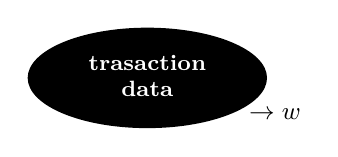
\begin{tikzpicture}[baseline={([yshift=-.5ex]b.center)}]
      \node[ellipse,fill=black] (b){
        \textcolor{white}{\bf\footnotesize\begin{tabular}[c]{c}
                                            trasaction\\
          data
        \end{tabular}}
    };
    \node[anchor=west] (w) at (b.south east) {\small\({}\to w\)};
    \end{tikzpicture}
  }
  \qquad
  \subfloat[Transaction copy (trivial erasure share)]{
    \es: \tx
    % \begin{tikzpicture}[baseline={([yshift=-.5ex]b.center)}]
    %   \phantom{
    %   \node[ellipse,fill=black] (b){
    %     \textcolor{white}{\bf\footnotesize\begin{tabular}[c]{c}
    %       blob\\
    %       of\\
    %       data
    %     \end{tabular}}
    %   };}
    % % https://texample.net/tikz/examples/torn-paper/
    % % ‼ make cute torn edges
    % \clip[fill] ([xshift=-1em]b.north east)
    % -- ([yshift=1em]b.south west)
    % -- ([xshift=1em]b.south west)
    % -- ([yshift=-1em]b.north east) -- cycle;
    % \node[ellipse,fill=black] (b){
    %     \textcolor{white}{\bf\footnotesize\begin{tabular}[c]{c}
    %       blob\\
    %       of\\
    %       data
    %     \end{tabular}}
    %   };
    % \end{tikzpicture}
}
  % \qquad
  % \subfloat[Worker \(y\) is commiting to the hash of~\(x\)]{
  %   \(y♯x\): \([\#(x)]_{\sim y}\)
  % }%‼

\subfloat[Batch hash of worker~\(w\)]{
  \#(\(\TXS\)):
  \#
    \(\left(\strut
          {\tx}:%\\%_{\to w}
          {\tx}:%\\%_{\to w}
          {\tx}:%\\%_{\to w}
          {\tx}:%\\%_{\to w}
          {\tx}:%\\%_{\to w}
          {\tx}%_{\to w}
          \right)\)
  }
  \subfloat[%
  Worker hash (broadcast by \(w\)),
  consisting of %
  the batch hash  \(\#\TXS\), %
  the batch number \(\bn\), %
  and the number of transactions \(\|\TXS\|\), %
  signed by~\(w\)]{
    \wh:
    \begin{tabular}[t]{@{}l@{}}
      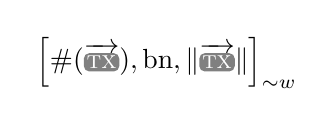
\begin{tikzpicture}[baseline={([yshift=-.5ex]wh.center)}]
        \node (wh){\(\left[ \#(\overrightarrow \tx), \bn,  \|\overrightarrow \tx\| \right]_{{\sim}w}\)};
      \end{tikzpicture}
      %\footnotesize
    % {\color{violet} + info for correctness checking} \\
    % (\eg number of \tx[s], or list of \#s)\\
    %   \emph{Tahoe – The Least-Authority Filesystem}
    \end{tabular}
  }

  \subfloat[Genesis Header]{
    \(\hd[]\):\(
\tikz[baseline={(x.base)}]{\node (x){
\(\left(p,\overrightarrow\wh\right)\)
};}\)
  }
\qquad
  \subfloat[Genesis certificate of availability]{
    \(\ac\):
    \(\Bigl[\hd[]\Bigr]_{\overrightarrow q}\)
  }

  \subfloat[Block]{
\bk:
    \begin{math}
      \left[\hd\right]_{\color{green!60!black}{\sim p_1 \dots \sim p_m} [ \color{green!60!black}\sim p_{m+1} \cdots \sim p_{k}]}
    \end{math}
  }
  \qquad
  \subfloat[Signed quorum]{
    \(\qs_p\):
    \begin{math}
      \begin{array}[c]{@{\rhd}l}
        [\bk_1 \cdots \bk_\ell]_{\sim p}
      \end{array}
    \end{math}
  }

  \subfloat[Header]{
    \(\hd\):\(
\tikz[baseline={(x.base)}]{\node (x){
\(\left(p,\overrightarrow\wh,\ac, \rnd, \overrightarrow {\#(\qsₚ)}\right)\)
};}\)
  }


  \caption{Overview of data structures}
  \label{fig:data-structures}

\end{figure}

\FloatBarrier

\section{Transaction life cycle}
\label{sec:trans-life-cycle}

A transaction goes through the following stages, %
first on the worker,
then on the primary,
finally off to execution.\xspace%
\endnote{%
  before going to bit Nirvana ...
}
In more detail, %
on a “sunny day”, %
the progress towards execution, step by step, %
is as follows: %
\begin{itemize}
\item
  submission to a worker, received as \tx←
\item
  the transaction gets assembled into a batch
  that is referenced by a worker hash, 
  which in turn is sent to the primary
  and received as \wh
\item
  the worker hash is included into a block header \hd
\item
  the block header is announced, received as \(\hd^*\)
\item
  the block header is provably available, 
  via reception of enough header signatures \(\hdₚ\)
\item
  the block header has reached integrity,
  via reception of enough header signatures \(\hdₚ\),
  \ie the transaction is now referenced by 
  a learner-specific block \bk
\item
  the block gets distributed
\item
  the block gets a quorum of signatures \qs
\item 
  eventually,\xspace%
  \footnote{%
    In fact, %
    this is the crucial point (see also \ref{??}). %
    % 
  } 
  the block gets commited,
  \begin{itemize}
  \item either if the signed quorum makes it into a leader block, 
  \item or by indirect reference
    (see \ref{...} for more detail)
    \todo{how do we do weak links anyway ... }
  \end{itemize}
\item
  the block containing the transaction gets executed. 
\end{itemize}
\todo{describe in more detail execution
  ... once we have that fixed
}

\section{Comparison with Narwhal}
\label{sec:comp-narwhal}
Let us see how the special case of a single learner amounts to %
a slightly more complicated version of Narwhal.
For workers nothing really chances.
Note that due to the restriction that a new block header %
has to contain at least one signed quorum (and at most one),
this means that every new header must contain a signed quorum;
moreover,
the signed quorum is a quorum of signatures for %
a previous block of the unique learner. %






\begin{theapx}
\appendix

\section{Learner graph jazz}
\ref{apx:learner-graph}

w.r.t.\ some specific other \base \(b\), %
thus giving rise to a learner-indexed family of collections of sets. %

The precise sense of what counts as big enough is rather simple:
for every pair of learner-specific quorums \(\q{a},\q{b}\), %
every ``safe'' set must intersect with both learner-specific quorums. %
Accordingly, %
the default setting for safety assumption is that 
we would suggest that learners use these derived sets that are just big enough
and thus are least likely to be proven wrong,
which might lead to all sorts of issues,
including forking.\xspace%
\todo{add footnote on how things go wring in detail}


: single-learner point of view

In particular, %
global weak quorums would be big enough. %

 such that 
\(a\) and \(b\), for each other \base \(b\); %
i.e., sets of validators that would aim for consistency between learners “own” \base \(a\) and any other \base \(b\).\footnote{%
  This includes the case where \(a=b\), %
  which amounts to asking for sets of non-Byzantine nodes. %
}

commit to a set of safe sets such that %
if at least one of its elements consists of correct validators only %
they expect to see agreement between \base[s] \(a\) and \(b\) %
provided that it also intersects non-trivially with %
every pair of qourums \(\q{a}\) and \(\q{b}\). %



\section{Message dependency management for actors}

\todo[inline,size=normalsize]{%
  possibly move to the main part of the  paper %
  although it is technically not needed for the high(est)-level spec
}
Messages depending on other messages %
is a \emph{sine qua non} of consensus protocols. %
Typically,
sending a message according to some protocol %
is a reaction to having received one or several messages.\xspace%
\footnote{%
  Elapsing timers act very much like “local messages” %
  (cf.\ \statetright's %
  \href{docs.rs/stateright/latest/stateright/actor/trait.Actor.html}%
  {\texttt{on\_tiemeout}}%
  ). 
}
However, %
high-level protocol descriptions do not---and \emph{should} not---specify %
how a process can effectively become aware of the fact that %
it should send a specific message, %
let alone how it should keep track of all relevant received messages (efficiently). %
However, %
if we want to run the protocol, % 
we {have to} address these questions
by implementing what we call \emph{message dependency management}. %
We shall follow the actor based model, % 
which means that we have to map high-level protocol descriptions like
\emph{upon reception of header signatures from a weak quorum of validators} %
to a function that the processes calls for \emph{every} single received message %
and returns  a set of messages to be sent. 
%This amounts to specifying an actor based implementation of the protocol. %
We shall explain that %
it was indeed appropriate to disregard questions of message dependency management
“without loss of generality” %
in our high-level description of \hnr. %

% When receiving a message, we have to first 
% the sender is aware of the fact that all messaged dependencies are met %
% and also can retrieve the received messages (from memory, storage, \etc). %
% Finally, %
% one has to have an efficient filter for irrelevant messages %
% (relative to the current observations of the agent). %

Let us look at some examples of message dependencies before %
we describe the complete message dependency manager.  %
\begin{ex}[Responses to header signature requests]
  Header signature requests (in the availability protocol)
  can only be answered (correctly) by a validator if
  it has received a confirmation from each of its workers.\footnote{
    Each confirmation states that
    a copy of the referenced transaction data has been stored.
  }
  This scenario is simple in that
  \begin{itemize}
  \item the primary knows exactly %
    which messages are expected from its workers; %
  \item each expected message's fingerprint is \emph{known in advance};
  \item there is only a single message to be synthesized and %
    it is known \emph{a priori}; % 
  \item progress towards meeting all dependencies is monotonic.
  \end{itemize}
  We can devise a relatively simple data structure:
  each expected message (fingerprint) is mapped to a pair of
  a shared counter and (a pointer to) the message to be signed.
  The counter is decremented of each one of the expected messages %
  and the message is synthesized. % 
\end{ex}

Now, if we look at availability certificates,
the situation becomes more tricky:
we are interested only in the first \(k\) messages out of \(n\);
moreover, 
the synthesized message depends on which messages turn out to be 
the first \(k\). 

\begin{ex}[Broadcasting certificates of availability (\textsc{i/ii})]
  Assuming that all validator sets of size~\(f+1\) (out of~\(3f+1\))
  form a weak quorum, we
  \begin{enumerate}
  \item count down a counter, starting from \(f+1\);
  \item synthesize the certificate of availability (and broadcast it)
    when the counter reaches \(0\);
  \item free the counter when it reaches~\(-2f\).
  \end{enumerate}
  There are optimizations to be made for the last point, 
  using a more efficient mechanism for identifying 
  messages that we can safely ignore. 
\end{ex}

In general, the situation becomes already a nightmare, %
if we consider fully general quorum systems. %
\todo[inline,size=normalsize]{%
  probably kick this example out. 
}
\begin{ex}[Broadcasting certificates of availability (\textsc{ii/ii})]
  \todo{the below works only for systems in there is a single node in every
    quorum -- a veto node
    alternatively, one could put things “upside down”,
    and let the leaves report on success -- 
    provided that every quorum has a node that does not belong to any other
    quorum (every neighborhood has a grumpy person)
  }\color{red}
  Assuming more general quorum systems,
  the idea of a simple counter does not work any more. %
  The brute force solution consists in using one counter for each quorum; %
  however, that would lead to an exponential blow-up. %
  Hence,
  we make use of the fact that
  each message falls into exactly one “region”\xspace%←that \xspace
  % allows do remove the footnote easily
  \footnote{%
    There is a one to one correspondence of regions and terms
    in the inclusion-exclusion formula,
    and \emph{vice versa}.
  }
  of the Venn diagram of all quorums. 
  Based on the
  \href{https://en.wikipedia.org/wiki/Inclusion\%E2\%80\%93exclusion_principle}%
  {inclusion exclusion principle}, %
  we can organize the regions of the Venn diagram (of a set of subsets of a set)
  into a tree in which
  \begin{itemize}
  \item the root is the region of elements that belong to all sets
  \item the leaves are the regions of elements that belong to exactly one set
  \item there is a path from one region to another if the former is contained in
    every set that the latter is contained in
  \item in particular, the elements of a direct ancestor belong to exactly one additional set.
  \end{itemize}
  We set up a system of counters,
  one for each non-empty region,
  initialized to the size of the region.
  Each received signature contributes to exactly one counter,
  which is decremented upon message delivery. 
  Now,
  we have received enough signatures if, and only if, 
  all counters on a branch reach zero.
 \endnote{%
 \emph{On the inclusion exclusion principle.} %
   We can simplify this tree by repeating the following two operations,
   starting at the root:
   \begin{enumerate}
   \item coalesce all children of the same cardinality 
   \item coalesce parent and child if the child is the only child
   \end{enumerate}
   For a proper counter system, %
   we can disregard empty regions; %
   moreover,
   we can disregard empty regions. 
   Thus,
   we need at most one counter per learner. 
   Finally,
   counters organize into a tree in a natural way
   such that
   we have received enough signatures if, and only if, 
   all counters on a branch reach zero.
   \\\centerline{
     \colorbox{Apricot}{%
       \begin{tabular}[c]{p{20em}}
         Does the above algorithm (up to some corner case details of empty regions)
         yield a single node if we start with the set of all sub-sets?
       \end{tabular}
     }
   }
}
\end{ex}

We discern the following sub-tasks of message dependency management: %
filtering, trigger detection, message synthesis, (local) state update. %
\begin{description}
\item[Filtering] %
  How we can efficiently sort out irrelevant messages? %
\item[Trigger detection] %
  Is the received message a trigger for sending new messages?
\item[Message retrieval] %
  How can we retrieve exactly the relevant received messages?
\item[State update] %
  Update the local state for the above three processes to work. %
\end{description}
In fact, %
we update the state not in one single action, %
but divide it maintaining %
a “database” of messages on the one hand %
and accompanying triggering information on the other hand. %
Each trigger might result in a state update;
there may be a cascade of triggers
where, at least intuitively,
the triggered effect result in triggering new effects. %

\todo[inline,size=normalsize,caption={}]{%
  revise this after going once through the protocol,
  filling descriptions of message dependencies
}


\begin{figure}[htb]
  \centering
  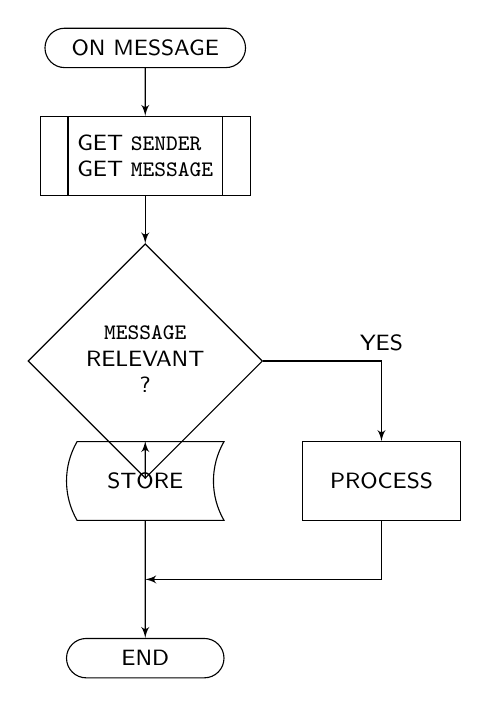
\begin{tikzpicture}[>=latex',font={\sf \footnotesize}]
      \def\smbwd{2cm}
      \node (terminal1) at (0,0) [draw, terminal,
      minimum width=\smbwd,
      minimum height=0.5cm] {ON MESSAGE};
      \node[below=4ex of terminal1] (predproc1) [%
      draw,%
      predproc,%
      align=left,%
      minimum width=\smbwd,%
      minimum height=1cm] {%
        GET \texttt{SENDER}\\%
        GET \texttt{MESSAGE}%
      }; 
      \node[below=4ex of predproc1] (decide1) [%
      draw, decision,
      minimum width=\smbwd,
      minimum height=1cm] {%
        \begin{tabular}[c]{@{}c@{}}%
          \texttt{MESSAGE}%
          \\%
          RELEVANT%
          \\?%
        \end{tabular}%
      };
      \node (storage1) at (0,-5.5) [draw, storage,
      minimum width=\smbwd,
      minimum height=1cm] {STORE};
      \node (process1) at (3,-5.5) [draw, process,
      minimum width=\smbwd,
      minimum height=1cm] {PROCESS};
      \coordinate (point1) at (0,-6.75);
      \node (terminal2) at (0,-7.75) [draw, terminal,
      minimum width=\smbwd,
      minimum height=0.5cm] {END};
      \draw[->] (terminal1) -- (predproc1);
      \draw[->] (predproc1) -- (decide1);
      \draw[->] (decide1) -| node[above]{YES} (process1);
      \draw[->] (decide1) -- (storage1);
      \draw[->] (process1) |- (point1);
      \draw[->] (storage1) -- (point1) -- (terminal2);
  \end{tikzpicture}
  \caption[Message dependency management]{Message dependency management:
    top-level flow chart}
  \label{fig:msg-dep-mng}
\end{figure}

In the accompanying %
\href{https://github.com/anoma/typhon/tree/hnarwhal-stateright}%
{prototype implementation}, %
these tasks are accomplished %
inside \statetright's \texttt{on\_msg}-functions. %


\begin{verbatim}
{
from [37] L. Zheng. Making distributed computation secure by construction. PhD thesis,
Cornell University, Ithaca, New York, USA, Jan. 2007.
}

4.4 Replication and message synthesis

Replicating code and data is an effective way to achieve
fault tolerance and ensure integrity and availability.
In DSR, both reactors and memory references may be replicated
on multiple hosts. Suppose reactor c is replicated on a set of hosts H.
Then other reactors interact with c as follows:
• Any message for c is sent to all the hosts in H.
• The replicas of c process incoming messages independently of each other. To
make this possible, all the program states of c have a local copy on every host in H.
In particular, every memory reference (location) accessed by c is also replicated
on H.
• If invoked with the same context identifier, the replicas of c are supposed to pro-
duce the same messages. Thus, the receiver host h of such a message µ may
receive the replicas of µ from different hosts in H. The redundancy is crucial
for achieving fault tolerance. Some hosts in H may be compromised, and these
bad hosts may send corrupted messages or simply not send anything. In general,
the replicas of µ received by h contain some correct ones, which are the same,
and some bad ones, which can be arbitrarily inconsistent. It is up to h to identify
the correct µ from those message replicas. This process is called message syn-
thesis, and the algorithm for identifying the correct message is called a message
synthesizer.
\end{verbatim}

\begin{verbatim}
message synthesizer ref(s)
  [37] L. Zheng. Making distributed computation secure by construction. PhD thesis,
  Cornell University, Ithaca, New York, USA, Jan. 2007.

  [39] L. Zheng and A. C. Myers. A language-based approach to secure quorum replication.
  In Proceedings of the Ninth Workshop on Programming Languages and Analysis for
  Security, PLAS’14, pages 27:27–27:39, New York, NY, USA, 2014. ACM. ISBN
  978-1-4503-2862-3. . URL http://doi.acm.org/10.1145/2637113.2637117.
\end{verbatim}



  
\end{theapx}
\begin{theendnotes}

\section{Endnotes}
\printendnotes

\end{theendnotes}


\todo[author=YourName]{%   
  Your “PR” here
}

\printbibliography
\end{document}

%%% -output-format=dvi ← for externalizing dvis instead of pdfs
%%% Local Variables:
%%% mode: latex
%%% TeX-master: t
%%% TeX-engine: luatex
%%% TeX-command-extra-options: "-shell-escape"
%%% End:
